\documentclass[10.5pt,notitlepage]{article}
\usepackage[utf8]{inputenc}
\usepackage{amsthm}
\usepackage{amsmath}
\usepackage{amsfonts}
\usepackage{mathtools}
\usepackage{amsmath,amssymb}       
\usepackage{enumitem}   
\usepackage{enumerate}
\usepackage{verbatim} 
\usepackage{bbm}
\usepackage{booktabs}
\renewcommand{\qedsymbol}{$\blacksquare$}
\usepackage{makecell}
\usepackage[spanish]{babel}
\decimalpoint
\usepackage[letterpaper]{geometry}
\usepackage{mathrsfs}
\newenvironment{solucion}
  {\begin{proof}[Solución]}
  {\end{proof}}
\pagestyle{plain}
\usepackage{pdflscape}
\usepackage[table, dvipsnames]{xcolor}
\usepackage{longtable}
\usepackage{tikz}
\def\checkmark{\tikz\fill[scale=0.4](0,.35) -- (.25,0) -- (1,.7) -- (.25,.15) -- cycle;} 
\usepackage[bottom]{footmisc}
\usepackage{hyperref}
\usepackage{float}
\usepackage[utf8]{inputenc}
\usepackage{bbm}
\usepackage{placeins}
\newcommand{\pp}{\mathbb{P}}
\newcommand{\BB}{\mathcal{B}}
\newcommand{\RR}{\mathbb{R}}
\newcommand{\FF}{\mathcal{F}}
\newcommand{\CC}{\mathcal{C}}
\newcommand{\oo}{\varnothing}
\newcommand{\ee}{\varepsilon}
\newcommand{\NN}{\mathbb{N}}
\newcommand{\PP}{\mathcal{P}}
\newcommand{\LL}{\mathrm{L}}
\newcommand{\XX}{\mathbf{X}}
\newcommand{\xx}{\mathbf{x}}
\DeclareMathOperator{\Tr}{Tr}
\newcommand{\abs}[1]{\left\lvert #1 \right\rvert}
\newcommand{\norm}[1]{\left\| #1 \right\|}
\newcommand{\inner}[1]{\left\langle #1 \right\rangle}
\newcommand{\corch}[1]{\left[ #1 \right]}
\newcommand{\kis}[1]{\left\{ #1 \right\}}
\newcommand{\pare}[1]{\left( #1 \right)}

\theoremstyle{plain}

\newtheorem{thm}{Teorema}[section] % reset theorem numbering for each chapter
\newtheorem{defn}[thm]{Definición} % definition numbers are dependent on theorem numbers
\newtheorem{lem}[thm]{Lema} % same for example numbers
\newtheorem{remarkex}{Observación}
\newenvironment{rem}
  {\pushQED{\qed}\renewcommand{\qedsymbol}{$\triangle$}\remarkex}
  {\popQED\endremarkex}

\usepackage{geometry}
\usepackage{mathtools}
\usepackage{enumitem}
\usepackage{framed}
\usepackage{amsthm}
\usepackage{thmtools}
\usepackage{etoolbox}
\usepackage{fancybox}

\newenvironment{myleftbar}{%
\def\FrameCommand{\hspace{0.6em}\vrule width 2pt\hspace{0.6em}}%
\MakeFramed{\advance\hsize-\width \FrameRestore}}%
{\endMakeFramed}
\declaretheoremstyle[
spaceabove=6pt,
spacebelow=6pt
headfont=\normalfont\bfseries,
headpunct={} ,
headformat={\cornersize*{2pt}\ovalbox{\NAME~\NUMBER\ifstrequal{\NOTE}{}{\relax}{\NOTE}:}},
bodyfont=\normalfont,
]{exobreak}

\declaretheorem[style=exobreak, name=Ejercicio,%
postheadhook=\leavevmode\myleftbar, %
prefoothook = \endmyleftbar]{exo}
\usepackage{graphicx}
\graphicspath{ {images/} }
\title{Tarea 5: Modelos Estadísticos I.}

\author{Rojas Gutiérrez Rodolfo Emmanuel}

\date{\today}

\begin{document}

\maketitle

\begin{rem}
En los ejercicios 1,3 y 4 será necesario suponer la normalidad de los términos de error a través de los distintos modelos ajustados para obtener ciertas propiedades distribucionales\footnote{Además claro de independencia e idéntica distribución.}. En el ejercicio 2 se tendrá después de hacer cierto análisis, que este supuesto no es sostenible bajo un primer modelo, sin embargo bajo una modificación podría ser razonable.
\end{rem}
\setcounter{exo}{0}
\begin{exo}[Tiempos de entrega de refrescos]

    Un embotellador de refrescos analiza las rutas de servicio de las máquinas expendedoras en su sistema de distribución. Le interesa predecir el tiempo necesario para que el representante de ruta atienda las máquinas expendedoras en una tienda. Esta actividad de servicio  consiste en abastecer la máquina con productos embotellados y algo de mantenimiento o limpieza. El ingeniero industrial responsable del estudio ha sugerido que las dos variables más importantes que afectan el tiempo de entrega ($Y\,$) son la cantidad de cajas de producto abastecido ($X_1$) y la distancia recorrida por el representante ($X_2$). El ingeniero ha reunido 25 observaciones de tiempo de entrega que se muestran en la tabla \ref{tab 1}.
     \begin{itemize}
        \item[a)] Haga un análisis de regresión lineal, considerando la variable respuesta $Y$ y las variables predictivas. Comente el resultado del análisis.
        \item[b)] Encuentre la correlación simple entre las cajas ($X_1$) y la distancia $(X_2)$.
        \item[c)] Encuentre los factores de inflación de la varianza.
        \item[d)] Encuentre el número de condición de la matriz $X$.
        \item[e)] De acuerdo a (b, c y d), ¿considera que hay evidencia de multicolinealidad en estos datos?
     \end{itemize}
\end{exo}
 \begin{table}[htbp]
        \caption{Datos del problema de entrega de refrescos. $Y$ es el tiempo de  entrega, $X_1$ es el número de cajas y $X_2$ es la distancia recorrida.}
        \centering\begin{tabular}{@{}l@{\hskip 0.3in}r@{\hskip 0.3in}r@{\hskip 0.3in}r@{}}
            \toprule
            $i$ & $X_{1i}$ & $X_{2i}$ & $Y_i$ \\
            \midrule
            1 & 7 & 560 & 16.68 \\
            2 & 3 & 220 & 11.50 \\
            3 & 3 & 340 & 12.03 \\
            4 & 4 & 80 & 14.88 \\
            5 & 6 & 150 & 13.75 \\
            6 & 7 & 330 & 18.11 \\
            7 & 2 & 110 & 8.00 \\
            8 & 7 & 210 & 17.83 \\
            9 & 30 & 1460 & 79.24 \\
            10 & 5 & 605 & 21.50 \\
            11 & 16 & 688 & 40.33 \\
            12 & 10 & 215 & 21.00 \\
            13 & 4 & 255 & 13.50 \\
            \bottomrule
        \end{tabular}
        \qquad\qquad
        \begin{tabular}{@{}l@{\hskip 0.3in}r@{\hskip 0.3in}r@{\hskip 0.3in}r@{}}
            \toprule
            $i$ & $X_{1i}$ & $X_{2i}$ & $Y_i$ \\
            \midrule
            14 & 6 & 462 & 19.75 \\
            15 & 9 & 448 & 24.00 \\
            16 & 10 & 776 & 29.00 \\
            17 & 6 & 200 & 15.35 \\
            18 & 7 & 132 & 19.00 \\
            19 & 3 & 36 & 9.50 \\
            20 & 17 & 770 & 35.10 \\
            21 & 10 & 140 & 17.90 \\
            22 & 26 & 810 & 52.32 \\
            23 & 9 & 450 & 18.75 \\
            24 & 8 & 635 & 19.83 \\
            25 & 4 & 150 & 10.75 \\ \\
            \bottomrule
        \end{tabular}
        \label{tab 1}
    \end{table}
\begin{solucion}
\noindent \textbf{a)} Lo primero que se hizo fue una Pairs Plot, figura \ref{fig:1}, debido a que se detectó la siguiente anomalía en los datos, observe que si se considera el caso en el que no tenemos cajas de producto que abastecer ni distancia que recorrer, esto es \(X_1 = X_2 = 0\), entonces la estimación del tiempo medio de entrega sería el intercepto de un hipotético modelo de regresión lineal, sin embargo, la estimación que más sentido hace en este caso es cero y por ende parecería ser que el modelo adecuado a considerar debería ser uno de regresión a través del origen.    
\begin{figure}[htb]
 \centering
 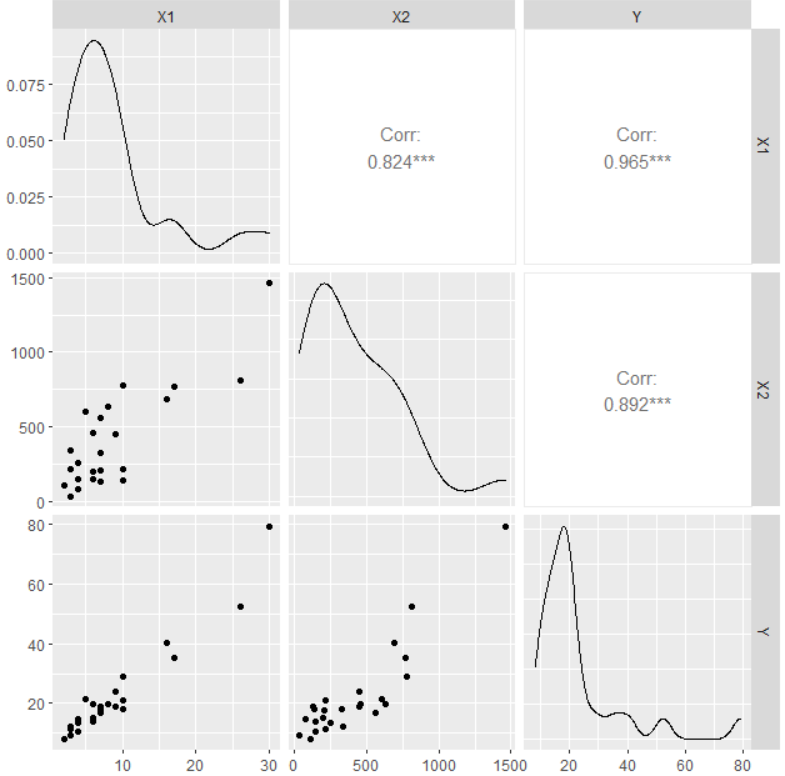
\includegraphics[scale = 0.65]{Ejercicio 1 Imagen 1 Pairs.png}
 \caption{Pairs Plot de los Datos Proporcionados.}
\label{fig:1}
\end{figure}
Sin embargo, en el panel que corresponde a la gráfica de dispersión de de la distancia recorrida contra el tiempo de entrega, \(X_2\) vs \(Y\) figura \ref{fig:1} panel (3,2), se observó que aunque es posible trazar una recta que pasará por el origen y se ajustará de cierta manera a los puntos esta debería tener una pendiente algo pronunciada, siendo que para los puntos más cercanos a \((0,0)\) parecería que una recta con una pendiente un poco más suave que no pasa por el origen ajustaría mejor. Bajo esta hipótesis se ajusto el modelo de regresión lineal
\begin{equation*}
    E[Y_{i}|X_{i2}] = \gamma_{0} + \gamma_{1}X_{i2}, \ i =1, \hdots,25. . 
\end{equation*}
Las estimaciones para el mismo se presentan en la tabla \ref{tab:ref1}
\begin{table}[H]
        \centering
        \begin{tabular}{@{}l@{\hskip 0.3in}r@{\hskip 0.3in}r@{\hskip 0.3in}r@{}}
            \toprule
            Coeficiente& Estimación & \(t\)-valor& \(p\)-valor \\
            \midrule
            \(\gamma_0\) & 4.962 &  2.123& 0.0448\\
            \(\gamma_1\) & 0.043 &  9.447& \(2.21\cdot10^{-9}\)\\ 
            \bottomrule
        \end{tabular}
        \caption{Resultados análisis de regresión: \(Y\) variable respuesta, \(X_2\) variable explicativa.}
        \label{tab:ref1}
\end{table}
en la misma se puede observar que el intercepto \(\gamma_0\) es significativo bajo un nivel de significancia del \(5\%\). Por otro lado, en la figura \ref{fig:2} es posible apreciar la recta estimada sobrepuesta a los datos observados. En está figura llama la atención que aún considerando un modelo con intercepto, cuya estimación resulto en un valor positivo y además la estimación de la pendiente también fue positiva, las bandas de predicción en algunos puntos arrojan como posibles valores tiempos negativos, situación que podría agravarse en caso de considerar un modelo sin intercepto.
\begin{figure}[htb]
 \centering
 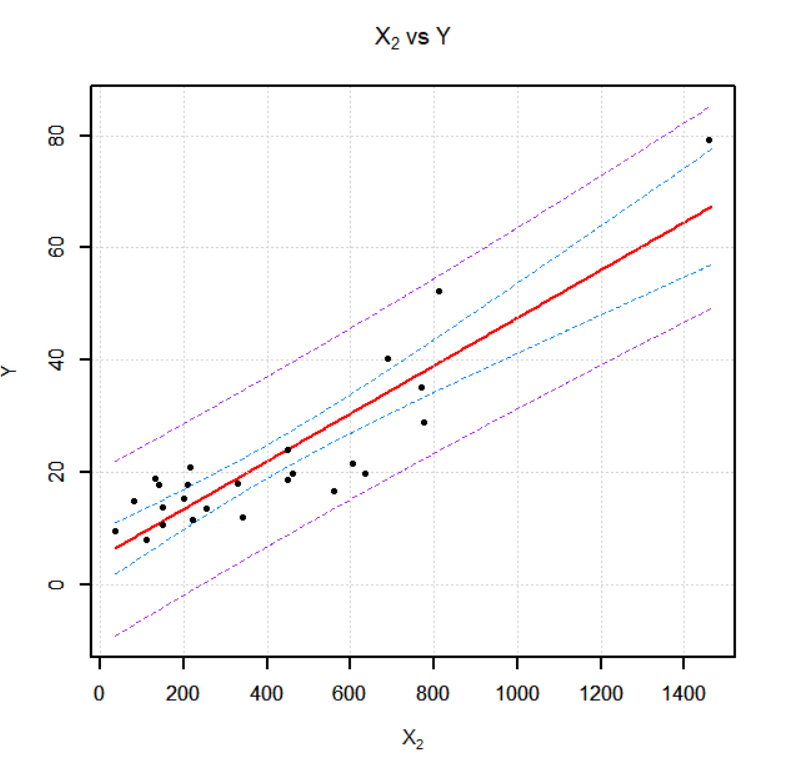
\includegraphics[scale = 0.65]{Ejercicio 1 Imagen 2 X2 vs Y.png}
 \caption{Recta de regresión para \(Y\) utilizando como única variable explicativa a \(X_2\). Observaciones en puntos negros, intervalo de confianza al \(95\%\) en linea punteada azul e intervalo de predicción al \(95\%\) en linea punteada púrpura.}
\label{fig:2}
\end{figure}
Como último paso para decidir que modelo se ajustaría a los datos, se realizaron las estimaciones correspondientes para ambos modelos de regresión, es decir
\begin{equation}\label{1.1}
        E[Y_{i}|X_{i1}, X_{i2}] = \beta_{01}X_{i1} + \beta_{02} X_{i2}, \ i =1, \hdots,25. 
\end{equation}
y 
\begin{equation}\label{1.2}
        E[Y_{i}|X_{i1}, X_{i2}] =\beta_{10} + \beta_{11}X_{i1} + \beta_{12}X_{i2}, \ i =1, \hdots,25.
\end{equation}
Se destaca que el modelo \eqref{1.1} obtuvo una \(R^2\) ajustada de \(0.9833\) y un AIC de \(137.536\), mientras que el modelo \eqref{1.2} obtuvo una \(R^2\) ajustada de \(0.9559\) y un AIC de \(134.830\). Dado que gráficamente pareciera ser que un intercepto debe ser considerado y dado que el modelo con intercepto \eqref{1.2} obtuvo un \(AIC\) menor, se eligió este para modelar el problema planteado, debido a que el modelo que no considera intercepto solo fue mejor respecto al \(R^2\) ajustada. Las estimaciones obtenidas para el modelo \eqref{1.2} se presentan en el cuadro \ref{tab:reg2}
\begin{table}[H]
        \centering
        \begin{tabular}{@{}l@{\hskip 0.3in}r@{\hskip 0.3in}r@{\hskip 0.3in}r@{}}
            \toprule
            Coeficiente& Estimación & \(t\)-valor& \(p\)-valor \\
            \midrule
            \(\beta_{10}\) & 2.341& 2.135&0.044\\
            \(\beta_{11}\) & 1.616&  9.464& \(3.25\cdot10^{-9}\)\\ 
            \(\beta_{12}\) & 0.014&  3.981& \(6.31\cdot10^{-4}\)\\
            \bottomrule
        \end{tabular}
        \caption{Resultados análisis de regresión: \(Y\) variable respuesta, \(X_1, X_2\) variables explicativas.}
        \label{tab:reg2}
\end{table}
Primeramente, se destaca que todos los coeficientes resultan significativos\footnote{Incluyendo al intercepto, lo que refuerza aún más la elección del modelo con intercepto.} bajo un nivel de significancia del \(5\%\), además recordando que estamos interesados en detectar colinealidad, esto último junto con el hecho de que el \(R^2\) ajustada para este modelo fue del \(0.9559\), es un buen primer indicio de que en caso de existir colinealidad la misma no es tan fuerte, ya que una de las primeras señales de colinealidad fuerte entre las variables independientes es un coeficiente de determinación alto, con valores \(t\) que arrojen como resultado el que algunos coeficientes para las variables independientes no son significativamente distintos de cero. \\ 

\noindent \textbf{b) } La correlación lineal simple entre la cantidad de cajas de producto abastecido ($X_1$) y la distancia recorrida por el representante ($X_2$) es:
\begin{equation}\label{1.5}
    \rho_{12} = \frac{\sum_{i=1}^{25}(X_{i2} - \overline{X_2})(X_{i1} - \overline{X_1})}{\sqrt{\sum_{i=1}^{25}(X_{i2} - \overline{X_2})^2\sum_{i=1}^{25}(X_{i1} - \overline{X_1})^2}} = 0.824. 
\end{equation}
Lo cual coincide con la correlación arrojada en la Pairs Plot \eqref{fig:1} para estos valores, esta correlación parece un poco alta considerando que el valor de la misma siempre se encuentra entre \([-1,1]\) y una correlación lineal exacta se da con un valor de \(1\)\footnote{O una correlación lineal exacta pero inversa, se da con un valor de \(-1\).}. Sin embargo, no podemos concluir la existencia de colinealidad fuerte entre las variables independientes únicamente basándonos en este indicador, más aún, recordando que el inciso anterior nos dio resultados esperanzadores en este aspecto. \\ 

\noindent \textbf{c)} Los factores de inflación de la varianza se obtuvieron de acuerdo con Rawlings, Applied Regression Analysis a Research Tool, utilizando los elementos de la diagonal de la inversa de la matriz de correlación de \(X_1\) con \(X_2\). Del inciso anterior se deduce que la matriz de correlación de \(X_1\) con \(X_2\) es:
\begin{equation*}
 R_{12} = \begin{pmatrix}
 1.000& 0.824\\ 
 0.824& 1.000
 \end{pmatrix},
\end{equation*}
la cual tiene por inversa a 
\begin{equation*}
 R_{12}^{-1} = \begin{pmatrix}
  3.118& -2.570\\ 
 -2.570& 3.118
 \end{pmatrix}. 
\end{equation*}
De este modo, los factores de inflación de la varianza quedan dados por
\begin{equation}\label{1.12}
    VIF_{1} = VIF_{2} = 3.118.
\end{equation}
Nuevamente de acuerdo a Rawlings, Applied Regression Analysis a Research Tool, se puede concluir que los resultados presentados en \eqref{1.12} resultan esperanzadores, ya que el hecho de que los factores de inflación de la varianza sean menores que \(10\) indican que no hay evidencia de una colinealidad fuerte entre las variables independientes\footnote{De hecho ni siquiera pasan el \(5\) que es el primer punto donde podría haber alerta de colinealidad.}. Otra manera de calcular estos factores es recordando que 
\[
VIF_{i} = \frac{1}{1 - R_{i}^2}, \ i= 1,2,
\]
donde \(R_{i}^2,\ i=1,2\) es el coeficiente de determinación resultante de correr una regresión lineal simple con \(X_i\) como respuesta y la otra variable independiente como regresora. En este caso, de lo probado en la \textbf{Tarea 2 Ejercicio 3}, se tiene que \(R_{i}^2 = \rho_{12}^2 = 0.679, \ i = 1,2\), haciendo los cálculos de esta manera se llega al mismo resultado que en \eqref{1.12} y resulta más claro el porque un valor alto para el factor de inflación\footnote{Observando que entre mas cercano sea \(\rho_{12}\) a uno o menos uno, más grande serán estos factores.}, resulta en una colinealidad fuerte entre las variables.\\ 

\noindent \textbf{d)} 
Sea \(X = \begin{pmatrix}1' &X_1 & X_2 \end{pmatrix}\) la matriz de datos para este problema, donde \(1'\) es un vector columna de \(25 \times 1\) con unos en todas sus entradas. Para calcular el número de condición de \(X'X\) se obtuvieron los valores singulares de \(X'X\), luego denotando por \(\sigma_{\max}(X'X)\) al máximo de ellos y \(\sigma_{\min}(X'X)\) al mínimo, se utilizó el hecho de que el número de condición \(K(X'X)\) esta dado por 
\begin{equation}\label{condi}
    K(X'X) = \frac{\sigma_{\max}(X'X)}{\sigma_{\min}(X'X)}= \frac{6.728\cdot10^{6}}{8.819}= 762957.3.
\end{equation}
Este número de condicionamiento es alto y podría parecer alarmante, debido a que un número de condicionamiento alto implica que existirán problemas numéricos al invertir la matriz \(X'X\), pero que tanto están relacionados estos problemas numéricos con colinealidad entre las columnas de \(X\). De acuerdo con Belsley y Kuh el considerar números de condicionamiento en matrices cuyas columnas tienen escalas muy distintas, puede ocasionar que dichos números se vean fuertemente afectados a causa de las diferentes escalas, por esto proponen calcular dicho numero de condición escalando cada una de las columnas de la matriz objetivo de tal modo que todas sus columnas tengan longitud uno. Bajo este criterio se tiene que el número de condición de una matriz, calculado como el cociente entre su mayor valor singular y su menor valor singular es siempre mayor o igual a uno, y alcanza el valor de \(1\) solamente cuando las columnas de la matriz escalada son ortogonales, es decir cuando la colinealidad es prácticamente inexistente. Por ende, números de condición que rebasen por mucho la unidad indicaran que la matriz que esta siendo evaluada esta cada vez más 'alejada' de una matriz cuyas columnas no presentan multicolinealidad alguna. Sea \(\tilde{X}\) el escalamiento de la matriz \(X\) tal que sus columnas tienen longitud igual a uno, se obtuvo que 
\begin{equation}\label{condi2}
    K(\tilde{X}) = 6.378. 
\end{equation}
Pero que tan alejado es este valor de \(1\), puede consultarse en Rawlings que \ref{condi2} es una cota superior de los denominados índices de condicionamiento para la matriz \(\tilde{X}\), los cuales indican que hay colinealidad moderada entre las columnas de \(X\) cuando alguno de ellos supera el valor de \(30\), dado que en este caso \eqref{condi} es igual a \(6.378\) es imposible que algún índice de condicionamiento sea mayor a \(30\) y por ende, se tiene otro indicador de que la colinealidad entre las columnas de \(X\), que parece existir por la correlación obtenida en el \textbf{inciso b)} de este ejercicio, es más bien débil. \\ 

Por último, se tomó el siguiente criterio por recomendación del profesor sea \(\mathcal{X} = \begin{pmatrix} X_1 & X_2 \end{pmatrix}\) la matriz que contiene como columnas a los distintos valores de las variables independientes \(X_1\) y \(X_2\), y sea ahora \(\tilde{\mathcal{X}}\) la matriz resultante de centrar y escalar las columnas de \(\mathcal{X}\), entonces se procede a calcular el número de condicionamiento para la matriz \(\tilde{\mathcal{X}}'\tilde{\mathcal{X}}\) como 
\begin{equation}\label{vale kk}
    K(\tilde{\mathcal{X}}'\tilde{\mathcal{X}}) = \frac{\lambda_{\max}}{\lambda_{\min}} = \frac{0.517}{9.44\cdot 10^{-2}}=5.474,
\end{equation}
donde \(\lambda_{\max}\) y \(\lambda_{\min}\) representan al valor propio mas grande y al valor propio más pequeño\footnote{Los cuales coinciden con los valores singulares en este caso.}, de la matriz \(\tilde{\mathcal{X}}'\tilde{\mathcal{X}}\). Debido a que dicho número de condicionamiento es menor a \(100\), entonces tiene otro indicador de que la colinealidad que pueda existir entre las variables independientes es más bien débil.\\ 

\noindent \textbf{e)} De acuerdo a lo realizado en los incisos anteriores, vimos que cierta colinealidad podría existir debido a que la correlación muestral entre \(X_1\) y \(X_2\) parecía ser algo alta, de hecho echando una vistazo a la gráfica de dispersión entre \(X_2\) y \(X_1\) presentada en la figura \ref{fig:1} pareciera verse marcada cierta relación lineal. A pesar de ello, tanto el número de condicionamiento \eqref{condi2} tomado de las recomendaciones de Belsley y Kuh, como el número de condicionamiento obtenido mediante las recomendaciones del profesor \eqref{vale kk}, los factores de la inflación de la varianza y lo comentado sobre el análisis de regresión presentado en \ref{tab:reg2}, nos indican que dicha colinealidad es débil o lo más moderada.
\end{solucion}


%%%%%%%%%%%%%%%%%%%%%%%%%%%%%%%%%%%%%%%%%%%%%%%%%%%%%%%%%%%%%%%%%%%%%%%%%%%%%%%%%%%%%%%%%%%%%%%%%%%%%%%%
\begin{exo}
    Para el conjunto de los datos de la tabla \ref{tab 2} haga lo siguiente.
    \begin{itemize}
        \item[a)] Ajuste el modelo de regresión lineal simple.
        \item[b)] ¿Los residuos son independientes o están autocorrelacionados? Haga una prueba gráfica y una prueba analítica (Durbin--Watson).
        \item[c)] En otros estudios similares a este, los residuos muestran un patrón de autocorrelación, siguiendo un proceso autoregresivo de orden 1. Por tal razón, haga el análisis, siguiendo un procedimiento tipo Cochran y Orcutt.
        \item[d)] Haga una prueba de independencia de los residuos que resultan del modelo corregido con el procedimiento de Cochran y Orcutt.
        \item[e)] Comente los resultados de los incisos anteriores.
    \end{itemize}
\end{exo}

    \begin{table}[htbp]
        \caption{Valores de las variables respuesta ($y$) y explicativa ($x$) del ejercicio 2.}
        \centering\begin{tabular}{@{}lr@{\hskip 0.4in}r@{}}
            \toprule
            Observación & $X$ & $y$ \\
            \midrule
            1 & 7.048 & 54.46 \\
            2 & 9.286 & 67.50 \\
            3 & 6.946 & 56.41 \\
            4 & 4.648 & 42.95 \\
            5 & 4.942 & 46.16 \\
            6 & 6.313 & 53.43 \\
            7 & 9.552 & 70.16 \\
            8 & 9.456 & 69.27 \\
            9 & 6.531 & 53.98 \\
            10 & 4.681 & 47.09 \\
            11 & 3.060 & 39.33 \\
            12 & 9.313 & 67.98 \\
            13 & 8.214 & 62.48 \\
            14 & 3.932 & 41.18 \\
            15 & 6.462 & 55.52 \\
            16 & 6.048 & 52.56 \\
            17 & 4.660 & 46.27 \\
            18 & 8.509 & 64.80 \\
            19 & 2.684 & 37.74 \\
            20 & 8.675 & 65.72 \\
            \bottomrule
        \end{tabular} 
        \qquad\qquad
        \begin{tabular}{@{}lr@{\hskip 0.4in}r@{}}
            \toprule
            Observación & $X$ & $y$ \\
            \midrule
            21 & 8.381 & 65.14 \\
            22 & 0.411 & 31.50 \\
            23 & 0.965 & 33.68 \\
            24 & 8.785 & 70.51 \\
            25 & 9.893 & 75.25 \\
            26 & 1.909 & 32.28 \\
            27 & 2.211 & 30.54 \\
            28 & 7.659 & 59.05 \\
            29 & 8.944 & 64.81 \\
            30 & 8.967 & 60.29 \\
            31 & 6.957 & 51.65 \\
            32 & 8.725 & 56.93 \\
            33 & 8.807 & 56.81 \\
            34 & 9.898 & 66.27 \\
            35 & 0.411 & 18.95 \\
            36 & 8.986 & 61.50 \\
            37 & 4.483 & 40.16 \\
            38 & 4.800 & 40.79 \\
            39 & 9.812 & 65.04 \\
            40 & 8.593 & 57.20 \\
            \bottomrule
        \end{tabular}
        \label{tab 2}
    \end{table}
\begin{solucion}
\noindent \textbf{a)} Se ajustó un modelo de regresión lineal de la forma 
\begin{equation}\label{momomo}
    E[y_{i}|X_{i}] = \beta_{0} + \beta_{1}X_{i}, \ i = 1\hdots,40. 
\end{equation}
Las estimaciones por mínimos cuadrados para el modelo \eqref{momomo} así como algunos otros datos relacionados con ellas se muestran en el cuadro \ref{tab:reg3}
\begin{table}[H]
        \centering
        \begin{tabular}{@{}l@{\hskip 0.3in}r@{\hskip 0.3in}r@{\hskip 0.3in}r@{}}
            \toprule
            Coeficiente& Estimación & \(t\)-valor& \(p\)-valor \\
            \midrule
            \(\beta_0\) & 23.870 & 16.53   &  \(<2\cdot10^{-16}\)\\ 
            \(\beta_1\) & 4.523  & 22.25   & \(<2\cdot10^{-16}\)\\ 
            \bottomrule
        \end{tabular}
        \caption{Resultados análisis de regresión: \(Y\) variable respuesta, \(x\) variable explicativa.}
        \label{tab:reg3}
\end{table}
La última columna de la tabla en el cuadro \ref{tab:reg3} indica que los \(p\)-valores de las pruebas \(t\) correspondientes fueron menores a \(<2\cdot10^{-16}\), por ende ambos coeficientes resultan significativos bajo un nivel de significancia del \(5\%\). El \(R^2\) ajustada y el \(AIC\) para este modelo fueron 
\begin{equation}\label{Raju y aic 1}
    R^{2}_{adj} = 0.9268, \quad AIC = 220.764.
\end{equation}
Los valores anteriores nos ayudaran a comparar este modelo con uno que será ajustado más adelante. Por último, se deja en la figura \ref{fig:3} una gráfica de la recta de regresión ajustada encimada a los datos, con bandas de predicción y confianza al \(95\%\).\\ 
\begin{figure}[htb]
 \centering
 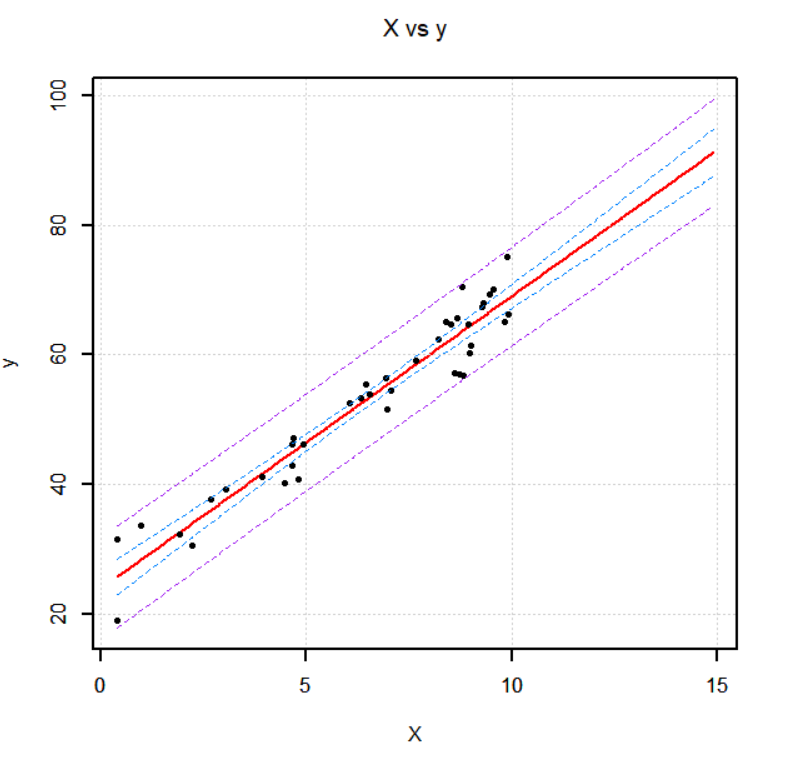
\includegraphics[scale = 0.65]{Ejercicio 2 Imagen 1 X vs y.png}
 \caption{Recta de regresión para \(y\) utilizando como variable explicativa a \(X\). Observaciones en puntos negros, intervalo de confianza al \(95\%\) en linea punteada azul e intervalo de predicción al \(95\%\) en linea punteada púrpura.}
\label{fig:3}
\end{figure}

\noindent \textbf{b)} Denote por \(e_i, i = 1,\hdots,40\) a los residuales de este modelo. En la figura \ref{fig:4} se presenta una gráfica de los residuales del tipo \(e_{i}\) contra \(e_{i-1}\) con \(i = 2, \hdots 40\). En dicha gráfica se nota un patrón creciente en los puntos graficados, por lo que parece existir una marcada correlación positiva entre los residuales.\\ 

\begin{figure}[htb]
 \centering
 \includegraphics[scale = 0.65]{Ejercicio 2 Imagen 2 ei vs ei{-1}.png}
 \caption{Gráfica del \(i\)-ésimo residual vs el residual inmediato anterior.}
\label{fig:4}
\end{figure}
Por otro lado, con ayuda del paquete \(tseries\) de \(R\) se realizó una gráfica de la función de autocorrelación de los residuales figura \ref{fig:5}. Las lineas horizontales azules son bandas de confianza del \(95\%\), la altura de las barras negras verticales correspondiente al valor \(k\) corresponde a la correlación entre el residual \(i\) y el residual \(i-k\), se omite la primer barra de la gráfica porque esta siempre es de tamaño \(1\). Que las barras se encuentren dentro de las bandas de confianza implica que esa correlaciones pueden ser consideradas como \(0\) con \(95\%\) de confianza, sin embargo se nota que la barra correspondiente a la correlación entre \(e_{i}\) y \(e_{i - 1}\) se sale por mucho de nuestras bandas, confirmando que existe correlación positiva y distinta de \(0\) entre estos términos. 
\begin{figure}[htb]
 \centering
 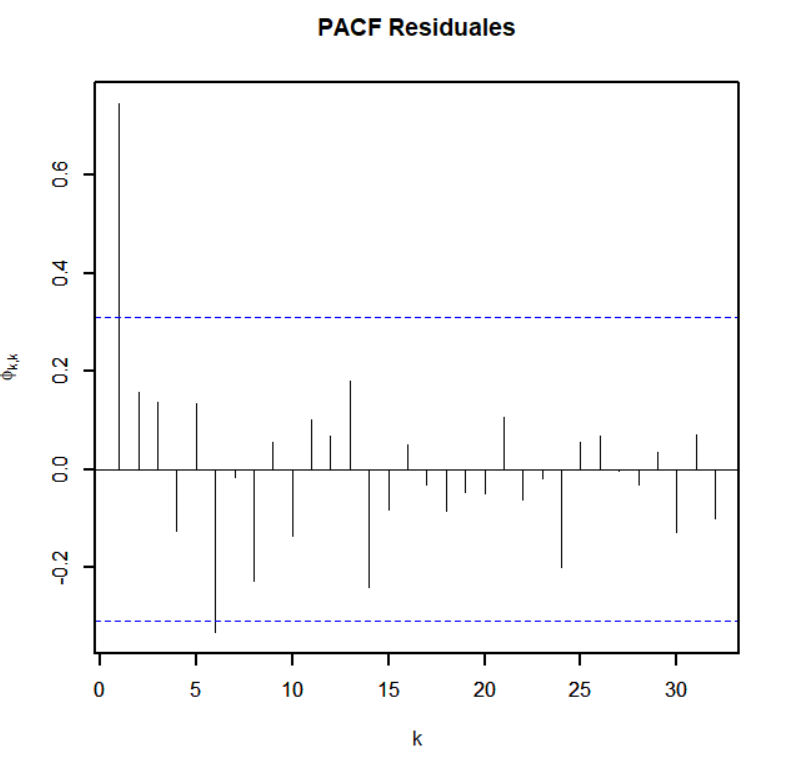
\includegraphics[scale = 0.65]{Ejercicio 2 Imagen 3 PACF Res 1.png}
 \caption{Gráfica de autocorrelación parcial de los residuales para el modelo de regresión lineal simple ajustado. Intervalo de confianza al \(95\%\) en linea punteada azul.}
\label{fig:5}
\end{figure}
Por último, se realizo la prueba de \(Durbin-Watson\), para ello se calculo el estadístico de la misma de acuerdo a la fórmula
\begin{equation}\label{estadistico chidori}
    d = \frac{\sum_{i = 2}^{40}(e_{i} - e_{i-1})^2}{\sum_{i = 1}^{40} e_{i}^2} = 0.444. 
\end{equation}
Este estadístico nos sirve para realizar dos pruebas de hipótesis acerca de la correlación \(\rho\), entre \(e_{i}\) y \(e_{i-1}\). La que se realizará es la prueba de hipótesis \(H_{0}: \rho = 0\) contra \(H_{1}: \rho > 0\), debido a que se sospecha la existencia de correlación positiva. Para ello es necesario obtener los valores críticos para la misma los cuales pueden encontrarse en la páginas \(631\) y \(632\) del libro de Rawlings, Applied Regresion Analysis a Research Tool, y se presentan en el cuadro \ref{tab:Durbin1}
\begin{table}[H]
        \centering
        \begin{tabular}{@{}l@{\hskip 0.3in}r@{\hskip 0.3in}r@{}}
            \toprule
            Nivel de significancia& \(d_{L}\) & \(d_{U}\) \\
            \midrule
            \(5\%\) & 1.39   & 1.60   \\ 
            \(1\%\) & 1.20   & 1.40  \\ 
            \bottomrule
        \end{tabular}
        \caption{Valores críticos para la prueba de hipótesis.}
        \label{tab:Durbin1}
\end{table}
Observe que bajo cualquiera de los dos niveles de significancia\footnote{La prueba rechaza \(H_0\) si \(d < d_{L}\), no rechaza \(H_0\) si \(d > d_{U}\) y es inconclusiva en otro caso.} se tiene que \( 0.44=d < d_{L}\), por lo que se rechaza la hipótesis nula \(H_{0}: \rho = 0\) bajo cualquiera de estos dos niveles de significancia, corroborando lo ya comentado de manera gráfica hasta el momento.\\ 

\noindent \textbf{c)} De acuerdo con las notas de clase, el procediento de Cochrane-Orcutt comienza suponiendo que los residuales del modelo original \eqref{momomo} siguen un proceso autoregresivo de primer orden (AR(1)), sin intercepto esto es 
\begin{equation*}
    e_i = \rho e_{i-1} + \xi_i, \ \abs{\rho} < 1.
\end{equation*}
Luego por mínimos cuadrados\footnote{En este caso deberían ser restringidos por la condición \(\abs{\rho} < 1\).} se obtiene una estimación de para \(\rho\) denotada por \(\hat{\rho}\), la cual fue calculada y esta dada por \(\hat{\rho} = 0.794\). Usando este valor se transforma el modelo \eqref{momomo} de la siguiente manera
\begin{equation}\label{mememe}
    E[y_{i} - \hat{\rho} y_{i-1}|X_{i} , X_{i-1}]  = \alpha(1 - \hat{\rho}) + \beta(X_{i} - \hat{\rho}X_{i - 1}) + \xi_{i}. \ i = 2, \hdots, 40.
\end{equation}
donde \(\xi_{i}\) es ruido blanco\footnote{Es decir los errores son \(i.i.d\) de media cero y varianza constante, esto se cumple siempre que el supuesto sobre los residuos del modelo original sea correcto.}. Posteriormente se estiman los coeficientes de \eqref{mememe} utilizando el procedimiento de mínimos cuadrados. Las estimaciones obtenidas se presentan en el cuadro \ref{tab:reg4}
\begin{table}[H]
        \centering
        \begin{tabular}{@{}l@{\hskip 0.3in}r@{\hskip 0.3in}r@{\hskip 0.3in}r@{}}
            \toprule
            Coeficiente& Estimación & \(t\)-valor& \(p\)-valor \\
            \midrule
            \(\alpha\) & 21.317 & 12.82 & \(3.51\cdot10^{-15}\) \\ 
            \(\beta\) &  4.849 & 55.17 & \(< 2\cdot10^{-16}\)\\ 
            \bottomrule
        \end{tabular}
        \caption{Resultados análisis de regresión: Modelo transformado utilizando el procedimiento de Cochrane–Orcutt.}
        \label{tab:reg4}
\end{table}
Nuevamente todos los coeficientes resultan significativos bajo un nivel de significancia del \(5\%\). Por otro lado, el \(R^2\) ajustada y el \(AIC\) para este modelo se presentan a continuación
\begin{equation*}
    R^{2}_{adj} =0.9909 \quad AIC = 163.728.
\end{equation*}
En ambos casos se nota una clara mejoría respecto a sus homónimos para el modelo \eqref{momomo} los cuales se presentaron en \eqref{Raju y aic 1}. Por último, se deja una gráfica de la recta de regresión para el modelo transformado con los datos transformado encimados, y las correspondientes bandas de confianza y predicción al \(95\%\) en la figura \ref{fig:4.5} \\
\begin{figure}[htb]
 \centering
 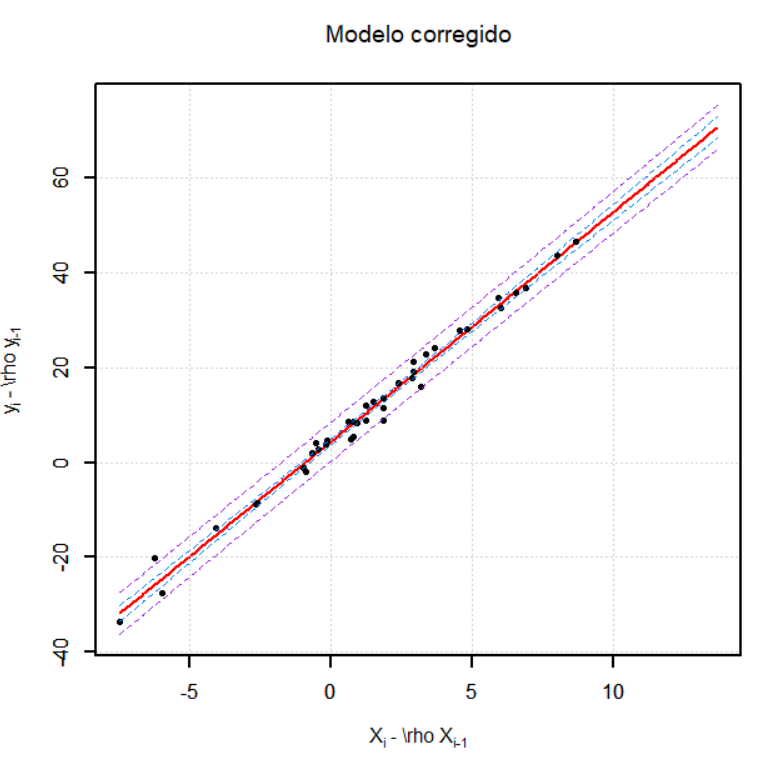
\includegraphics[scale = 0.65]{Ejercicio 3 Imagen chale.png}
 \caption{Recta de regresión para el modelo transformado. Observaciones en puntos negros, intervalo de confianza al \(95\%\) en linea punteada azul e intervalo de predicción al \(95\%\) en linea punteada púrpura.}
\label{fig:4.5}
\end{figure}

\begin{comment}
  También se incluye en la figura \ref{fig:6} una gráfica de comparación entre la recta estimada para el modelo \eqref{momomo}, con los coeficientes en el cuadro \ref{tab:reg3}, esto es 
  \[
   \widehat{E}[y_{i}|X_{i}] = 23.870 + 4.523X_{i}, \ i = 1\hdots,40. 
  \]
  Y la misma recta pero usando como estimación para los coeficientes los obtenidos por el procedimiento de Cochrane-Orcutt, es decir\\
  \[
   \widehat{E}[y_{i}|X_{i}] = 21.686 + 4.846X_{i}, \ i = 1\hdots,40. 
  \]
  \begin{figure}[htb]
 \centering
 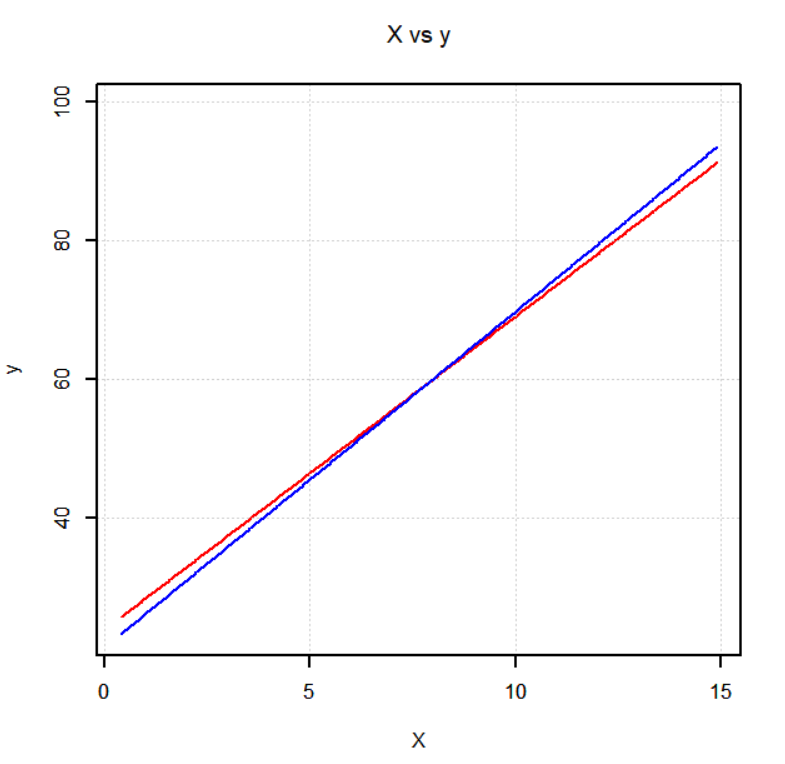
\includegraphics[scale = 0.65]{Ejercicio 2 Imagen 4 Coc & Orc.png}
 \caption{Rectas de regresión calculadas, en azul la obtenida mediante Cochrane-Orcutt, en rojo la recta de regresión lineal simple obtenida por MC.} 
\label{fig:6}
\end{figure}
\end{comment}

\noindent \textbf{d)}  Para este inciso denote por \(f_i\) a los residuales del modelos transformado \eqref{mememe}. Primero se realizó una gráfica de residuos \(f_i\) vs \(f_{i-1}\), como se hiciera en el modelo original, la cual se presenta en la figura \ref{fig:7}, en la misma se aprecia que el patrón creciente que se notaba en la gráfica de los residuales del modelo original \eqref{momomo} ha sido eliminado, y ahora la dispersión de los puntos parece más uniforme y sin ningún patrón evidente. \\
\begin{figure}[htb]
 \centering
 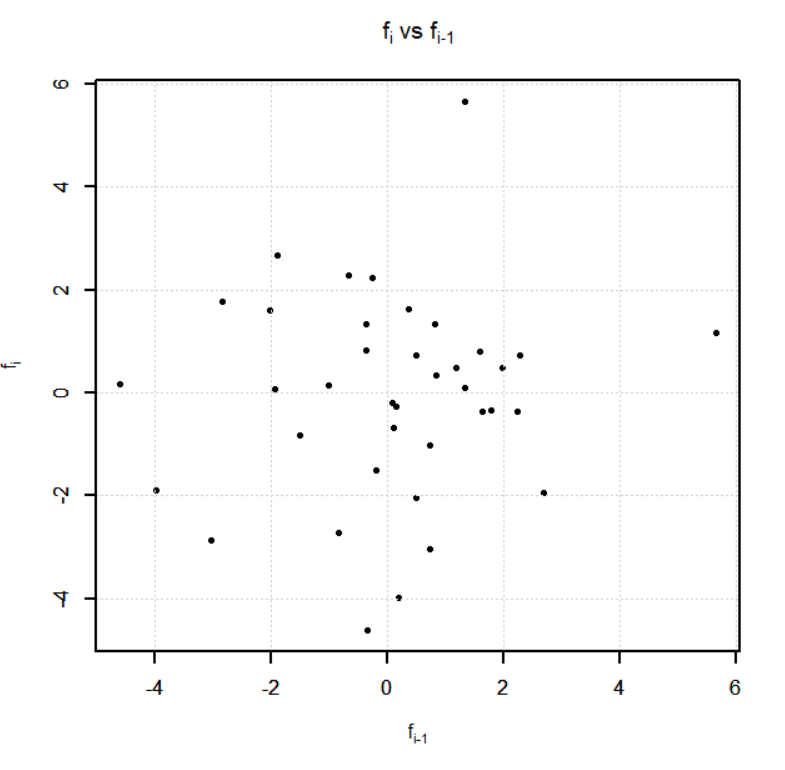
\includegraphics[scale = 0.65]{Ejercicio 2 Imagen 5 Res trans.png}
 \caption{Gráfica del \(i\)-ésimo residual del modelo transformado vs el residual inmediato anterior.}
\label{fig:7}
\end{figure}

Adicionalmente, se realizó la correspondiente gráfica de la función de autocorrelación de los residuos del modelo corregido, y en este caso se destaca que ya no hay ninguna barra que sobrepase en exceso las bandas de confianza, de hecho únicamente una de las barras cruza por poco al intervalo. 
\begin{figure}[htb]
 \centering
 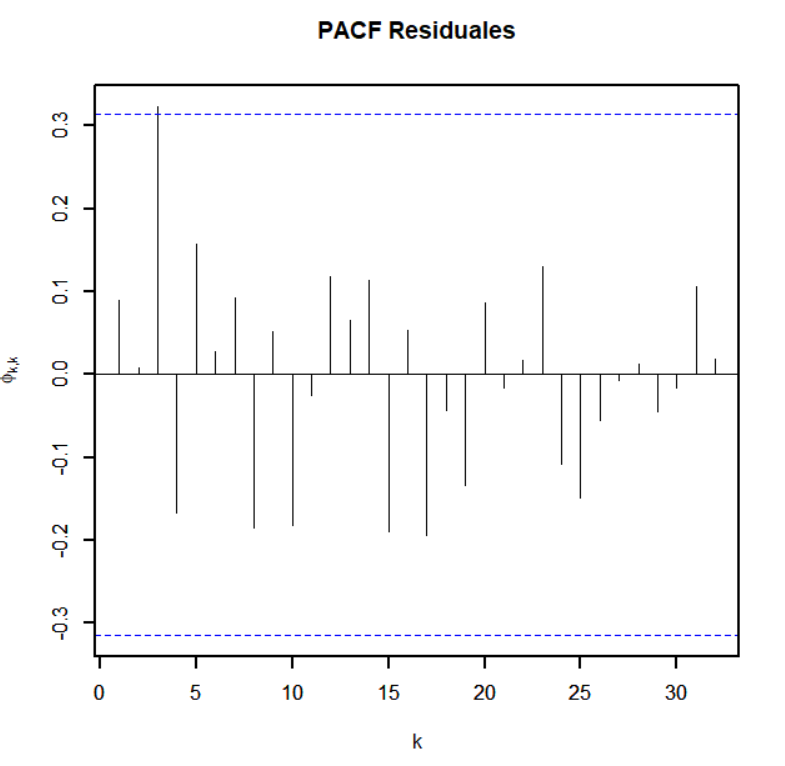
\includegraphics[scale = 0.65]{Ejercicio 2 Imagen 6 PACF Res trans.png}
 \caption{Gráfica de autocorrelación parcial de los residuales para el modelo obtenido por Cochrane-Orcutt. Intervalo de confianza al \(95\%\) en linea punteada azul.}
\label{fig:8}
\end{figure}
Por último, se realizó la prueba de Durbin Watson para el modelo corregido utilizando el estadístico 
\begin{equation}\label{durbinsito}
    d_f = \frac{\sum_{i = 2}^{39}(f_{i} - f_{i-1})^2}{\sum_{i = 1}^{39} f_{i}^2} =  1.744. 
\end{equation}
El cual se comparo con los valores críticos para la prueba\footnote{Donde \(\rho_f\) representa a la correlación entre \(f_i\) y \(f_{i-1}\).} \(H_0: \rho_f = 0\) contra \(H_1: \rho_f > 0\), los cuales se obtuvieron en la referencia mencionada con anterioridad y se muestran en el cuadro \ref{tab:Durbin2}
\begin{table}[H]
        \centering
        \begin{tabular}{@{}l@{\hskip 0.3in}r@{\hskip 0.3in}r@{}}
            \toprule
            Nivel de significancia& \(d_{L}\) & \(d_{U}\) \\
            \midrule
            \(5\%\) & 1.38   & 1.60   \\ 
            \(1\%\) & 1.19   & 1.39  \\ 
            \bottomrule
        \end{tabular}
        \caption{Valores críticos para la prueba de hipótesis.}
        \label{tab:Durbin2}
\end{table}
En ambos casos se constata que \(d_U < d_f = 1.744\) y por ende no hay evidencia suficiente para rechazar la hipótesis nula, bajo cualquiera de estos dos niveles de significancia. Por otro lado, restando a \(4\) el valor obtenido para \(d_f\) en \eqref{durbinsito} se obtiene el valor \(2.185\), este valor sirve para realizar el contraste de hipótesis \(H_0: \rho_f = 0\) contra \(H_1: \rho_f < 0\), utilizando los mismos valores críticos del cuadro \ref{tab:Durbin2} y el mismo criterio, observando entonces que \(2.256 = 4 - d_{f} > d_U\) en ambos casos, se concluye que tampoco es posible rechazar la hipótesis nula bajo estos niveles de significancia. Por lo comentado a lo largo de este inciso, se concluye que no hay evidencia estadística para pensar que los residuales del modelo corregido \eqref{mememe} estén autocorrelacionados.\\ 

\noindent \textbf{e)} A lo largo de este ejercicio observamos que los residuales del modelo original \eqref{momomo}, estaban correlacionados de manera positiva lo cual es un indicio de que el supuesto de terminos de error independientes puede no estarse cumpliendo. Dado que esta es una violación a los supuestos del modelo de regresión lineal, se esperaría un ajuste pobre del modelo a los datos, esto mismo se destacó una vez se resolvió el problema de los residuales usando el procedimiento de Cochrane-Orcutt, comparando medidas tales como los coeficientes de determinación ajustados y los \(AIC\) de los dos modelos ajustados en este ejercicio.  
\end{solucion}
%%%%%%%%%%%%%%%%%%%%%%%%%%%%%%%%%%%%%%%%%%%%%%%%%%%%%%%%%%%%%%%%%%%%%%%%%%%%%%%%%%%%%%%%%%%%%%%%%%%%%%%%
\begin{exo}
    Considere los datos de entrega de refrescos del problema 1. Haga lo siguiente.
    \begin{itemize}
        \item[a)] De las 25 observaciones que se muestran en la tabla \ref{tab 1}, determine cuáles son potencialmente influyentes. Argumente su respueta.
        \item[b)] Diga en cuales observaciones se tiene un mayor desplazamiento en la respuesta estimada ($\widehat{Y}_i$) cuando se hace la estimación eliminando dicha observación.
        \item[c)] Al observar los valores de la respueta $Y$ y las covariables $X_1$ y $X_2$, llaman la atención las observaciones 9 y 22, en las que hay que revisar su influencia. Haga un análisis de las observaciones 9 y 22, utilizando las métricas $DFBETAS_{ji}$ y $DFFITS_i$. Comente detalladamente sus hallazgos.
        \item[d)] ¿Cuáles observaciones deberían eliminarse en el análisis? ¿Por qué?
        \item[e)] Haga un análisis de residuos estudentizados y comente si los resultados de los incisos anteriores son acordes con el análisis de los residuos estudentizados.
    \end{itemize}
\end{exo}
\begin{solucion}
\noindent \textbf{a)} Para este inciso se utilizó la matriz de proyección del modelo calculado en el inciso \textbf{a) del ejercicio 1} tabla \eqref{tab:reg2}, de está se extrajeron los valores en su diagonal los cuales se denotaran por \(h_{ii}, \ i=1,\hdots,25\). En la figura \ref{fig:9} se puede apreciar una gráfica de estos valores contra el índice de la observación a la que corresponde cada uno de ellos, además de una linea en el valor de corte sugerido por Rawlings que es\footnote{Donde \(p=3\) es el número de parámetros en el modelo y \(n = 25\) es el número de observaciones en las que se baso el modelo.} \((2p)/n = 0.24\), las observaciones cuyo valor en la diagonal de la matriz de proyección sean mayor a este valor de corte se consideran, de acuerdo a este criterio, potencialmente influyentes. Se puede ver que en este caso únicamente dos de ellas rebasan dicho valor, dichas observaciones son la número \(9\) y la número \(22\) con un valor de \(0.498\) y \(0.392\) respectivamente.\\

\begin{figure}[htb]
 \centering
 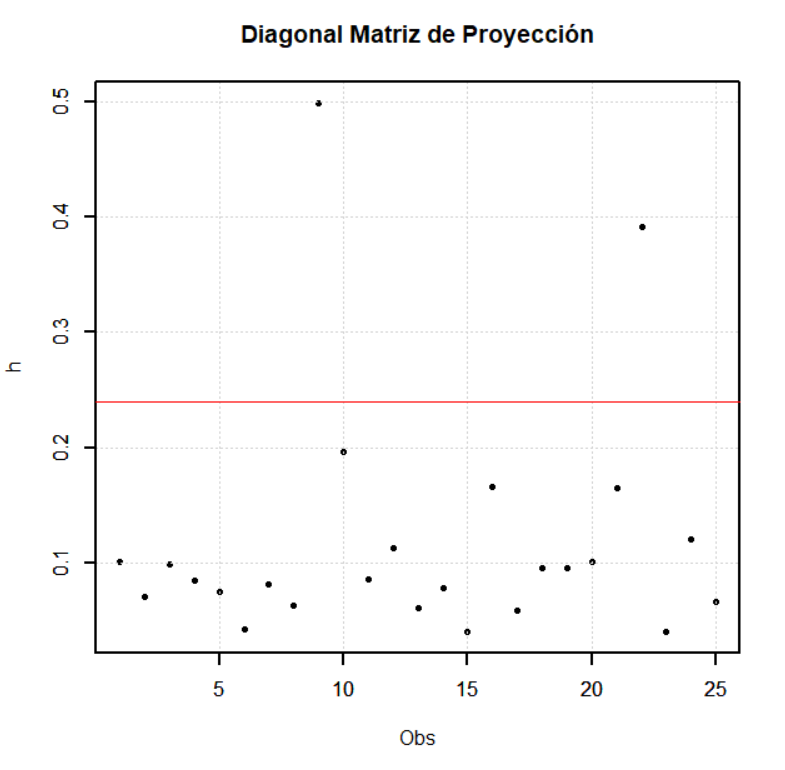
\includegraphics[scale = 0.65]{Ejercicio 3 Imagen 1 hii.png}
 \caption{Valores en la diagonal de la matriz de Proyección. La linea roja representa el valor de corte \((2p)/n =  0.24\).}
\label{fig:9}
\end{figure}

\noindent \textbf{b)} En la figura \ref{fig:chingatumadredembelé} vemos una gráfica del índice \(i\) contra la distancia entre el valor ajustado \(\hat{Y}_{i}\) y el valor ajustado \(\hat{Y}_{i(i)}\), donde este último representa al valor ajustado cuando la \(i\)-ésima observación no es considerada en el modelo. En puntos rojos se presentan los valores de esta distancia correspondientes a las observaciones número \(9\) y \(22\) que como puede notarse son las que mayor desplazamiento presentan en este aspecto. 
\begin{figure}[htb]
 \centering
 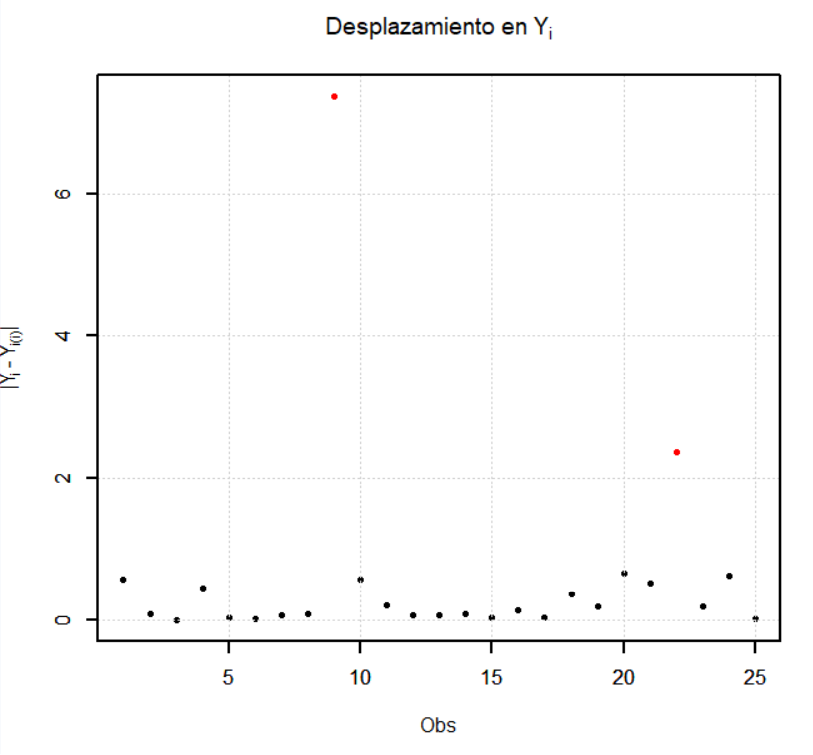
\includegraphics[scale = 0.65]{Desplazamiento.png}
 \caption{Valores de la \(D\) Cook para las distintas observaciones. Se resalta en puntos rojos las posibles observaciones influyentes obtenidas en el inciso anterior. La linea roja representa el valor de corte \(FQ_{0.5,p,n-p}\approx 0.814\).}
\label{fig:chingatumadredembelé}
\end{figure}
Por otro lado, el desplazamiento que se tiene en el vector de respuesta estimada al eliminar la observación \(i\) lo cuantifica la medida de influencia conocida como \(D\) de Cook. En la figura \ref{fig:10} se aprecia una gráfica del indice de las observaciones contra su correspondiente \(D\) de Cook \((D_i)\), los valores \(D_i\) se calcularon de acuerdo a la formula 
\begin{equation*}
    D_i = \frac{r_{i}^2}{p}\pare{\frac{h_{ii}}{1 - h_{ii}}},
\end{equation*}
donde \(r_i\) representa al \(i\)-ésimo residual estandarizado.  
\begin{figure}[htb]
 \centering
 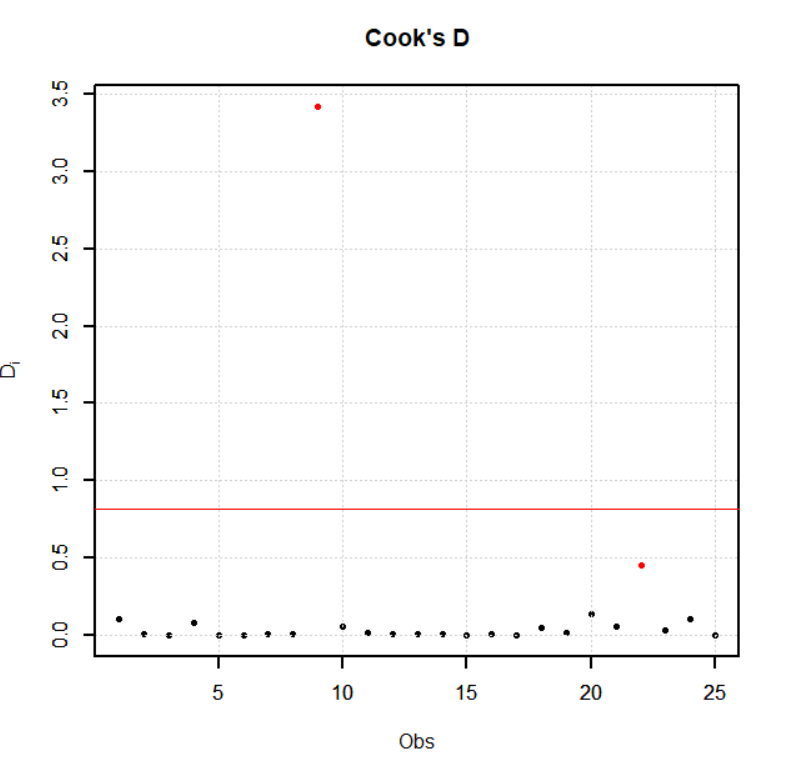
\includegraphics[scale = 0.65]{Ejercicio 3 Imagen 2 Cook's D.png}
 \caption{Valores de la \(D\) Cook para las distintas observaciones. Se resalta en puntos rojos las posibles observaciones influyentes obtenidas en el inciso anterior. La linea roja representa el valor de corte \(FQ_{0.5,p,n-p}\approx 0.814\).}
\label{fig:10}
\end{figure}
En la figura \ref{fig:10} se aprecia que las dos observaciones con mayor \(D_i\), y por tanto las que más influencia tienen en el desplazamiento de la respuesta al ser eliminadas, son nuevamente la número \(9\) y la número \(22\) en la gráfica estas observaciones aparecen como puntos rojos. Sin embargo, la linea roja que se aprecia en la gráfica mencionada es el valor de corte sugerido por Rawlings para determinar cuando este desplazamiento es suficientemente grande para considerar que hubo un gran cambio en la respuesta, debido a la eliminación de la observación correspondiente, para ello basta fijarse en aquellas observaciones cuya \(D_i\) rebase este valor. El valor de corte en este caso es el cuantil \(0.5\) de una distribución \(F\) con \(p = 3\) y \(n - p = 22\) grados de libertad el cual tiene un valor de \(0.814\). La \(D_i\) que rebasa con claridad dicho valor es la asociada a la observación \(9\) con un valor de \(3.419\), mientras que la segunda \(D_i\) con mayor valor es, como ya se mencionó, la asociada a la observación \(22\) con un valor de \(0.451\) sin embargo este valor esta aún algo lejos del valor de corte. En este sentido solo la observación \(9\) se considera potencialmente influyente en el desplazamiento de la respuesta cuando es eliminada.\\ 

\noindent \textbf{c)} Puede observar un gráfico de \(DFFITS_i\) en valor absoluto contra el índice de la observación a la que corresponde esta medida en la figura \ref{fig:11}. Rawlings menciona en su libro que otros autores como Belsley y Kuh, sugieren un valor de corte igual a \(2\sqrt{p/n} \approx 0.693\) a partir del cual las observaciones que tengan un valor de \(DFFITS_i\) mayor en valor absoluto al corte, serán consideradas influyentes bajo esta métrica. En la gráfica de la figura \ref{fig:11} dicho valor de corte esta representado por una linea horizontal en color rojo, igualmente en puntos rojos se indican los valores de esta métrica en valor absoluto asociados a las observaciones \(9\) y \(22\), los cuales en este caso son las únicos que rebasan la cota con un valor de \(4.296\) y \(1.195\) respectivamente.
\begin{figure}[htb]
 \centering
 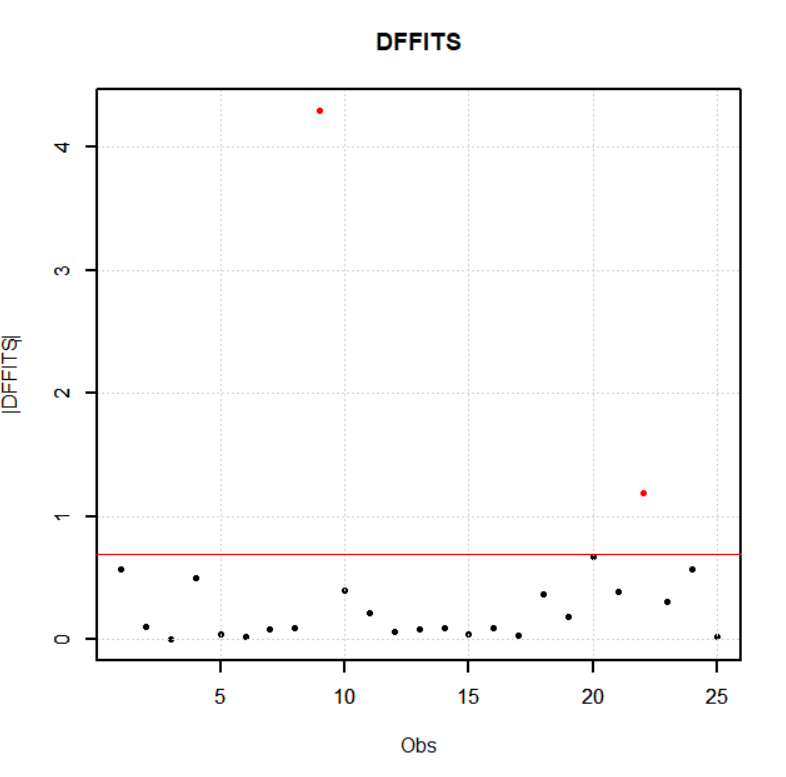
\includegraphics[scale = 0.65]{Ejercicio 3 Imagen 3 DFFITS.png}
 \caption{Valores de la medida \(DFFITS\) en valor absoluto para las distintas observaciones. Se resalta en puntos rojos las posibles observaciones influyentes obtenidas en el inciso anterior. La linea roja representa el valor de corte \(2\sqrt{p/n} \approx 0.693\).}
\label{fig:11}
\end{figure}
Por otro lado, en las figuras \ref{fig:12} a \ref{fig:14} se presentan las gráficas de las métricas \(DFBETAS_{(j)i}\) en valor absoluto contra los índices de las observaciones a la que corresponde dicha métrica, en todas ellas se representa con una linea horizontal en color rojo el valor de corte sugerido nuevamente por Belsley y Kuh el cual es \(2/\sqrt{n} = 0.4\), observaciones con valores mayores de \(DFBETAS_{(j)i}\) en valor absoluto a este valor de corte se consideran influyentes bajo está métrica. Se empezará comentando la gráfica en la figura \ref{fig:12} la cual corresponde a \(\abs{DFBETAS_{(0)i}} , \ i = 1,\hdots,25 \), está métrica nos dice que observaciones resultan más influyentes en la estimación del intercepto cuando las mismas son removidas para la estimación del modelo, nosotros estamos interesados en particular en los valores de está métrica en valor absoluto para las observaciones \(9\) y \(22\), los cuales se encuentran señalados como puntos rojos en la gráfica anterior, de ellos el único que rebasa con claridad el valor de corte es el asociado a la observación \(9\) con un valor de \(2.576\), a pesar de ello la métrica para la observación \(4\) en valor absoluto también rebasa por poco la cota establecida.\\ 
\begin{figure}[htb]
 \centering
 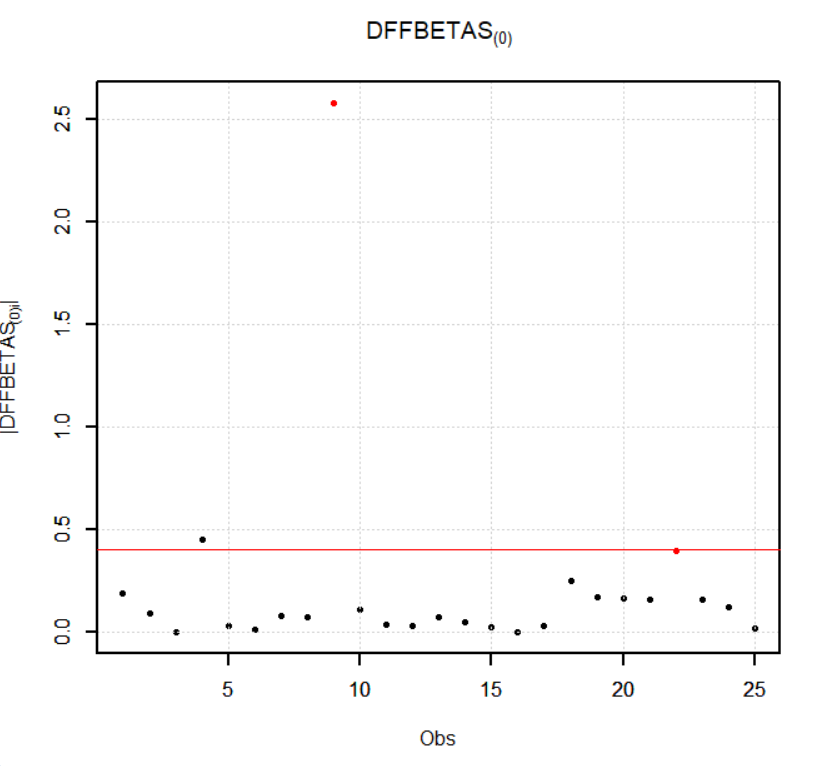
\includegraphics[scale = 0.65]{Ejercicio 3 Imagen 4 DBETAS 1.png}
 \caption{Valores de la medida \(DFBETAS\) en valor absoluto, para el intercepto, de las distintas observaciones. Se resalta en puntos rojos las posibles observaciones influyentes obtenidas en el inciso anterior. La linea roja representa el valor de corte \(2\sqrt{1/n} = 0.4\).}
\label{fig:12}
\end{figure}

Por otro lado, en la figura \ref{fig:13} se muestra la gráfica correspondiente a \(\abs{DFBETAS_{(1)i}} , \ i = 1,\hdots,25 \), está métrica nos dice que observaciones resultan más influyentes en la estimación del coeficente para la variable independiente \(X_1\),\footnote{Cantidad de cajas de producto abastecido.} cuando las mismas son removidas para la estimación del modelo. Nosotros estamos interesados en particular en los valores de está métrica en valor absoluto para las observaciones \(9\) y \(22\), los cuales se encuentran señalados como puntos rojos en la gráfica anterior, en este caso ambos rebasan con claridad el valor de corte con un valor de \(0.929\) y \(1.025\) respectivamente, a pesar de ello la métrica para la observaciones \(1\) y \(24\) en valor absoluto también rebasa por poco la cota establecida.\\ 
\begin{figure}[htb]
 \centering
 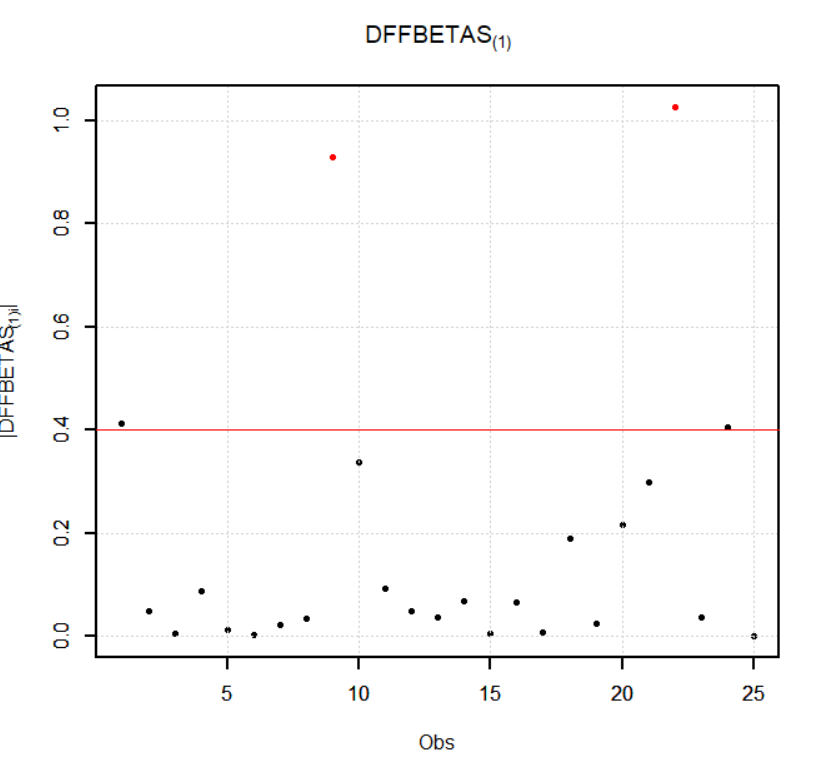
\includegraphics[scale = 0.65]{Ejercicio 3 Imagen 5 DBETAS 2.png}
 \caption{Valores de la medida \(DFBETAS\) en valor absoluto, para el coeficiente asociado a \(X_1\), de las distintas observaciones. Se resalta en puntos rojos las posibles observaciones influyentes obtenidas en el inciso anterior. La linea roja representa el valor de corte \(2\sqrt{1/n} = 0.4\).}
\label{fig:13}
\end{figure}

Por otro lado, en la figura \ref{fig:14} se muestra la gráfica correspondiente a \(\abs{DFBETAS_{(2)i}} , \ i = 1,\hdots,25 \), está métrica nos dice que observaciones resultan más influyentes en la estimación del coeficente para la variable independiente \(X_2\),\footnote{Distancia recorrida por el representante.} cuando las mismas son removidas para la estimación del modelo. Nuevamente, nosotros estamos interesados en particular en los valores de está métrica en valor absoluto para las observaciones \(9\) y \(22\), los cuales se encuentran señalados como puntos rojos en la gráfica anterior, en este caso ambos rebasan el valor de corte con un valor de \(1.508\) y \(0.573\) respectivamente, aunque únicamente el asociado a la observación \(9\) lo rebasa con claridad. A pesar de ello la métrica para la observaciones \(1\) y \(24\) en valor absoluto también rebasa por poco la cota establecida. \\ 
\begin{figure}[htb]
 \centering
 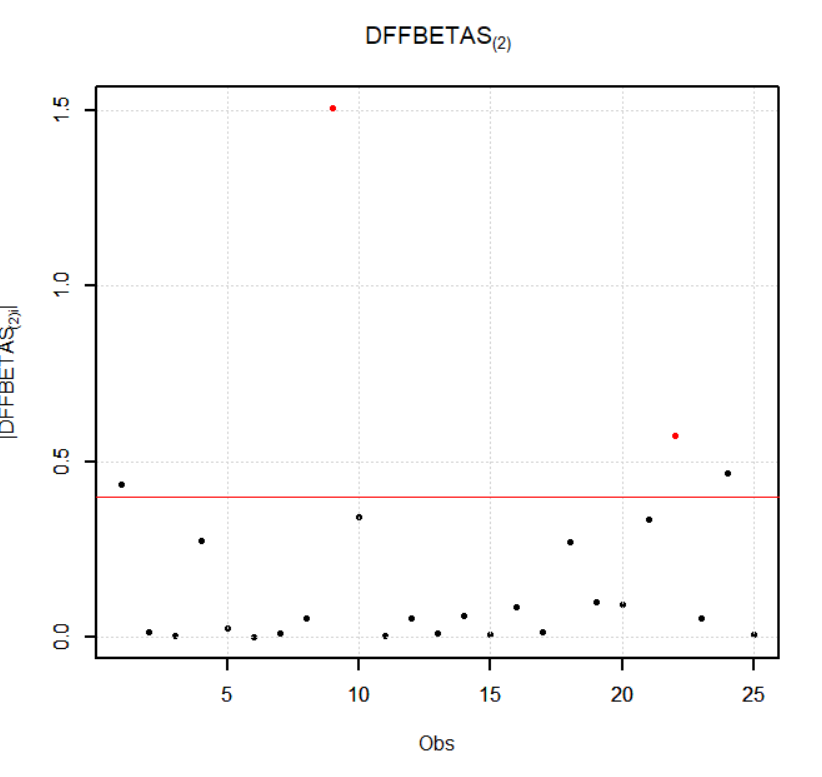
\includegraphics[scale = 0.65]{Ejercicio 3 Imagen 6 DBETAS 3.png}
 \caption{Valores de la medida \(DFBETAS\) en valor absoluto, para el coeficiente asociado a \(X_2\), de las distintas observaciones. Se resalta en puntos rojos las posibles observaciones influyentes obtenidas en el inciso anterior. La linea roja representa el valor de corte \(2\sqrt{1/n} = 0.4\).}
\label{fig:14}
\end{figure}

\noindet \textbf{d)} En los incisos anteriores se notó que la observación que más influye en diversos aspectos de la estimación del modelo, es la observación número \(9\) ya que influye tanto en el desplazamiento de la respuesta estimada, como en la estimación individual de cada uno de los coeficientes, por lo que se podría considerar eliminarla para realizar la estimación. Para tomar una decisión final se hizo una gráfica de dispersión las observaciones en la figura \ref{fig:15}
\begin{figure}[htb]
 \centering
 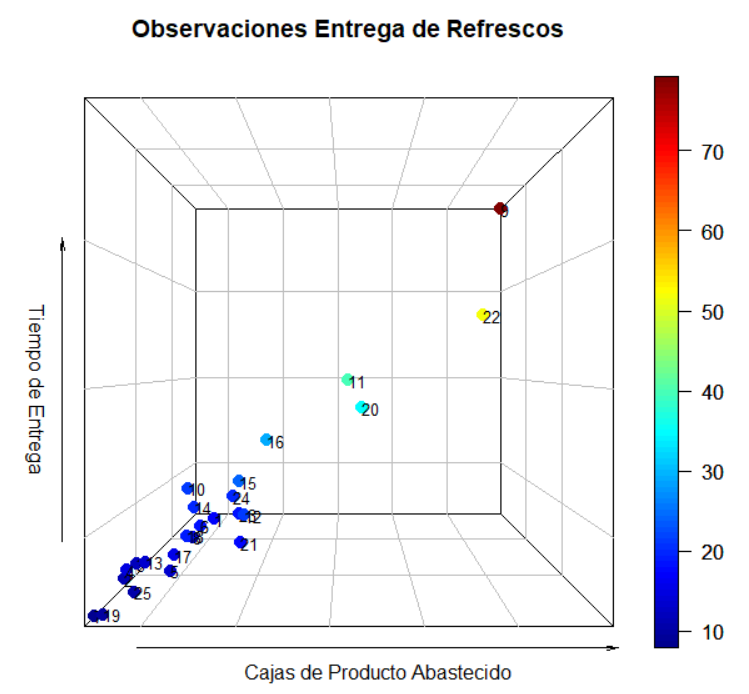
\includegraphics[scale = 0.65]{Ejercicio 3 Imagen 7 distancias.png}
 \caption{Datos en panorámica tridimensional con etiquetas numéricas. Se destaca que el punto en amarillo es la observación 22 y el punto en rojo intenso es la observación 9.}
\label{fig:15}
\end{figure}
En está gráfica se destaca con un punto en amarillo a la observación \(22\) y con punto en rojo intenso la observación \(9\). A pesar de que las observaciones \(9\) y \(22\) son las más alejada de la nube de puntos azules, lo que era de esperarse debido a su alto valor de  \(h_{ii}\), no parecen salirse mucho de la tendencia que llevan el resto de puntos. Por otra parte, se hicieron dos gráficas más en las que se encimó el plano de regresión estimado a la gráfica de dispersión de las observaciones, las misma se presentan en las figuras \ref{fig:16} y \ref{fig:17}. En ambas gráficas puede apreciarse que la observación \(9\) parece ser la más alejada al plano de regresión calculado y a los demás puntos, esto puede deberse simplemente a que la misma es un valor extremo pero posible, o quizás algún error de medición. Por lo que si se ha de eliminar una observación la mejor opción sería omitir la observación \(9\).\\
\begin{figure}[htb]
 \centering
 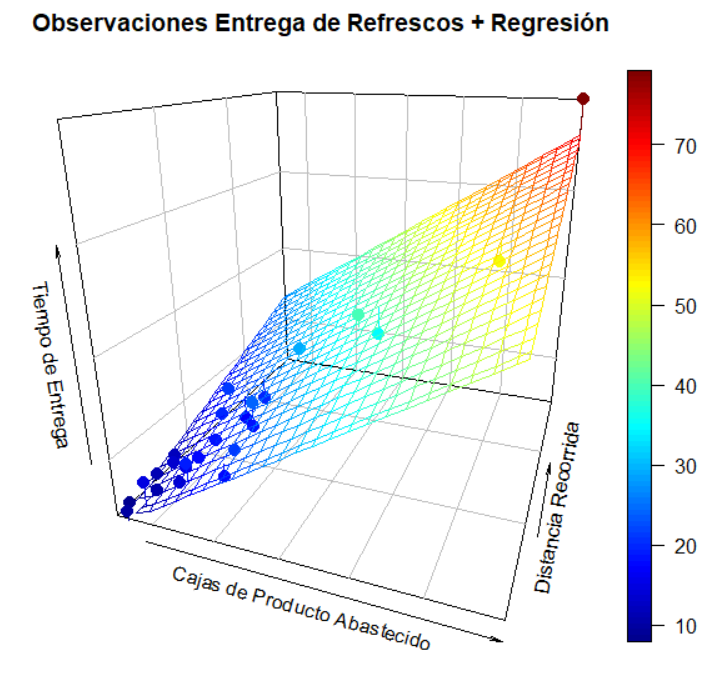
\includegraphics[scale = 0.65]{Ejercicio 3 Imagen 8 plano 1.png}
 \caption{Datos en panorámica tridimensional con plano de regresión lineal perspectiva 1. Se destaca que el punto en amarillo es la observación 22 y el punto en rojo intenso es la observación 9.}
\label{fig:16}
\end{figure}

\begin{figure}[htb]
 \centering
 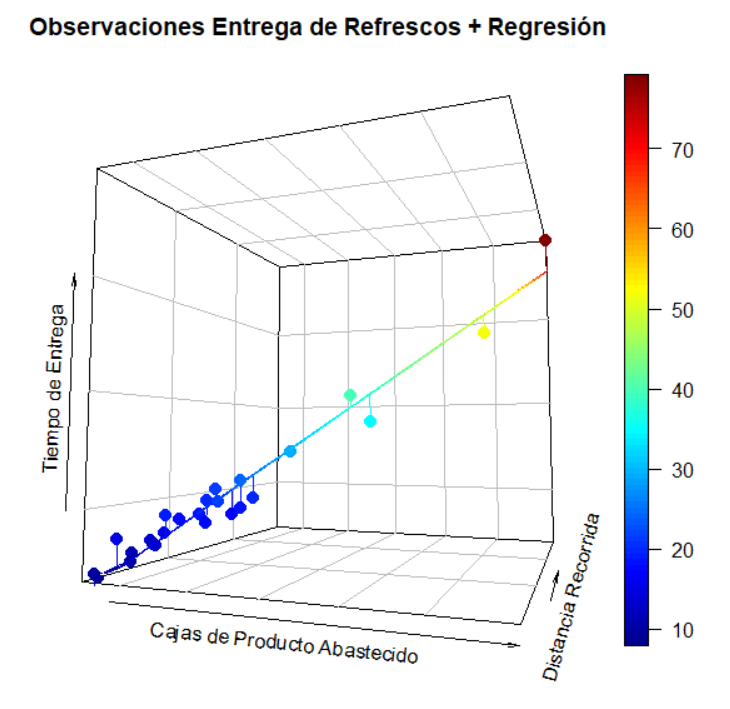
\includegraphics[scale = 0.65]{Ejercicio 3 Imagen 9 plano 2.png}
 \caption{Datos en panorámica tridimensional con plano de regresión lineal perspectiva 2. Se destaca que el punto en amarillo es la observación 22 y el punto en rojo intenso es la observación 9.}
\label{fig:17}
\end{figure}

\noindent \textbf{e)} Los residuales estudentizados se calcularon de acuerdo a la primer parte de esta tarea como
\begin{equation*}
    t_i = r_{i}\pare{\frac{n - p - 1}{n - p -r_{i}^2}}^{1/2}, \ i = 1,\hdots,25,
\end{equation*}
donde \(r_i\) es el \(i\)-ésimo residual estandarizado, dicho valores se distribuyen como una \(t(n- p -1)\) grados de libertad. Una gráfica de los residuales estudentizados contra su correspondiente valor ajustado se muestra en la figura  \ref{fig:17ups}, en lineas rojas se marcan los cuantiles \(0.025\) y \(0.975\) de una distribución \(t\) con \(n-p-1\) grados de libertad, y en puntos rojos se destacan los residuales estudentizados correspondientes a las observaciones \(9\) y \(22\), se destaca que el único de estos valores que se sale de este intervalo es el del residual asociado a la observación \(9\) con un valor de \(4.311\). Lo que corrobora lo hecho en los incisos anteriores.     
\begin{figure}[htb]
 \centering
 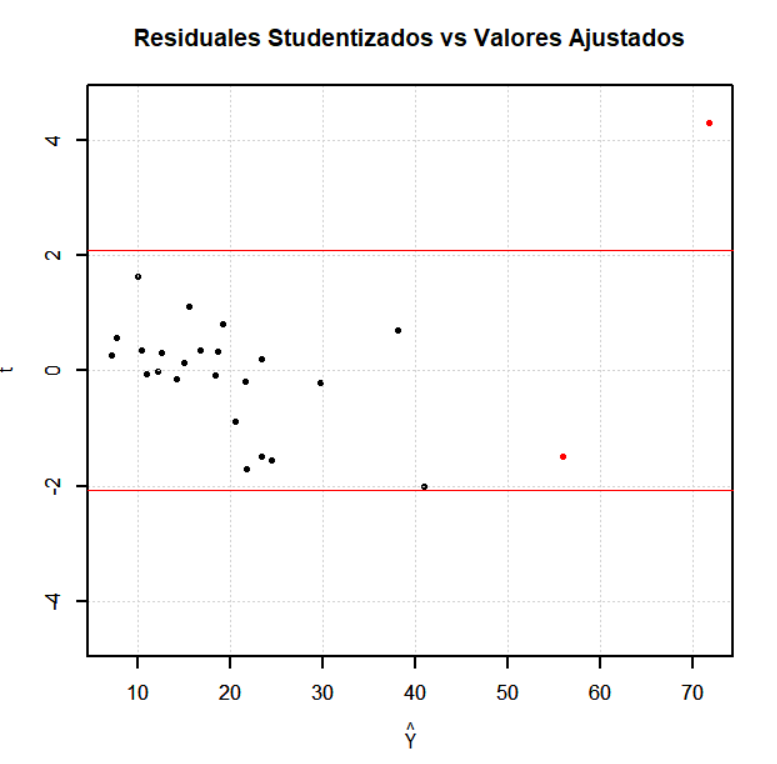
\includegraphics[scale = 0.65]{Ejercicio 3 Imagen 10 Student.png}
 \caption{Residuales estandarizados.}
\label{fig:17ups}
\end{figure}

\end{solucion}
%%%%%%%%%%%%%%%%%%%%%%%%%%%%%%%%%%%%%%%%%%%%%%%%%%%%%%%%%%%%%%%%%%%%%%%%%%%%%%%%%%%%%%%%%%%%%%%%%%%%%%%%
\begin{exo}
Suponga que una cadena de tiendas de un corporativo electrónico, que vende equipos y componentes electrónico, recopila información sobre las ventas anuales ($y$, medidas en miles de dólares), el número de casas que hay en el área de influencia de cada tienda ($x$, medida en millares) y la ubicación de la tienda (en colonia, en centro comercial y en zona centro). Mientras que la covariable $x$ es una variable continua, la covariable ubicación es una variable cuantitativa. En la tabla \ref{tab 3} se muestran los datos recopilados. Haga lo siguiente:
    \begin{itemize}
        \item[a)] Estime para cada una de las tres localizaciones (colonia, centro comercial y centro) los modelos de regresión lineal donde la respuesta es el volumen de ventas $y$ y la variable explicativa (continua) es el número de casas $x$.
        \item[b)] Haga una gráfica de dispersión del volumen de ventas ($y$) contra el número de casas en el área de influencia, para las tres localizaciones, utilizando tres caracteres gráficos diferentes, uno para cada localización. Sobreponga las rectas de regresión estimadas para cada una de las tres localizaciones. Comente la gráfica.
        \item[c)] Utilice en el modelo de regresión variables dummy y obtenga las diferencias entre los interceptos de las tres rectas estimadas (una por cada localización). Además del valor de la diferencia estimada presente su error estándar y comente si la diferencia es significativa.
        \item[d)] En los incisos anteriores asumimos que las rectas de regresión difieren solo en sus interceptos. ¿Cómo se puede investigar la diferencia entre las pendientes de las rectas? Investigue la diferencia entre las pendientes y comente los resultados
    \end{itemize}
\end{exo}
  \begin{table}[htbp]
        \caption{Datos de volúmens de ventas}
        \centering\begin{tabular}{@{}lrrr@{}}
            \toprule
            Tienda & Número de casas & Localización & Ventas \\
            \midrule
            1 & 161 & Colonia & 157.27 \\
            2 & 99 & Colonia & 93.28 \\
            3 & 135 & Colonia & 136.81 \\
            4 & 120 & Colonia & 123.79 \\
            5 & 164 & Colonia & 153.51 \\
            6 & 221 & CentroCom. & 241.74 \\
            7 & 179 & CentroCom. & 201.54 \\
            8 & 204 & CentroCom. & 206.71 \\
            9 & 214 & CentroCom. & 229.78 \\
            10 & 101 & CentroCom. & 135.22 \\
            11 & 231 & Centro & 224.71 \\
            12 & 206 & Centro & 195.29 \\
            13 & 248 & Centro & 242.16 \\
            14 & 107 & Centro & 115.21 \\
            15 & 205 & Centro & 197.82 \\
            \bottomrule
        \end{tabular}
        \label{tab 3}
    \end{table}
\begin{solucion}
\noindent \textbf{a)} Para este inciso se corrieron los tres modelos de regresión linea simple solicitados, utilizando a \(y\) el número de ventas anuales como la variable respuesta y a \(x\) el número de casas en la zona de influencia como variable explicativa. Los datos se separaron de acuerdo a la variable categórica Localización. Las estimaciones para cada uno de estos modelos se presentan en las tablas \ref{tab:reg10}-\ref{tab:reg12}  
\begin{table}[H]
        \centering
        \begin{tabular}{@{}l@{\hskip 0.3in}r@{\hskip 0.3in}r@{\hskip 0.3in}r@{}}
            \toprule
            Coeficiente& Estimación & \(t\)-valor& \(p\)-valor \\
            \midrule
            \(\beta_{0}^{Col}\) &  7.900& 0.511 & 0.644\\
            \(\beta_{1}^{Col}\) & 0.921 &  8.224  &\(3.76\cdot 10^{-3}\)\\ 
            \bottomrule
        \end{tabular}
        \caption{Resultados análisis de regresión ubicación colonia: \(E[y_{i}|x_{i}] = \beta_{0}^{Col} + \beta_{1}^{Col}x_{i}\), \(i \in \{1,\hdots,5\}\).}
        \label{tab:reg10}
\end{table}
\begin{table}[H]
        \centering
        \begin{tabular}{@{}l@{\hskip 0.3in}r@{\hskip 0.3in}r@{\hskip 0.3in}r@{}}
            \toprule
            Coeficiente& Estimación & \(t\)-valor& \(p\)-valor \\
            \midrule
            \(\beta_{0}^{CC}\) & 50.630&  2.918 & 0.062\\
            \(\beta_{1}^{CC}\) & 0.829 &   9.026& \(2.87\cdot 10^{-3}\)\\
            \bottomrule
        \end{tabular}
        \caption{Resultados análisis de regresión ubicación centro comercial: \(E[y_{i}|x_{i}] = \beta_{0}^{CC} + \beta_{1}^{CC}x_{i}\), \(i \in \{6,\hdots,10\}\).}
        \label{tab:reg11}
\end{table}
\begin{table}[H]
        \centering
        \begin{tabular}{@{}l@{\hskip 0.3in}r@{\hskip 0.3in}r@{\hskip 0.3in}r@{}}
            \toprule
            Coeficiente& Estimación & \(t\)-valor& \(p\)-valor \\
            \midrule
            \(\beta_{0}^{Cen}\) & 18.155 &  2.172& 0.118\\
            \(\beta_{1}^{Cen}\) & 0.887 &  21.794& \(2.11\cdot10^{-4}\) \\ 
            \bottomrule
        \end{tabular}
        \caption{Resultados análisis de regresión ubicación centro: \(E[y_{i}|x_{i}] = \beta_{0}^{Cen} + \beta_{1}^{Cen}x_{i}\), \(i \in \{11,\hdots,15\}\).}
        \label{tab:reg12}
\end{table}
En todos los casos se destaca que el intercepto no resulta ser significativamente diferente de cero bajo un nivel de significancia del \(5\%\), siendo los casos más extremos los de los modelos para las ventas hechas en la colonia y en el centro. A pesar de ello los valores de \(R^2\) ajustada de los modelos para las ventas de colonia, centro comercial y centro son \(0.943,0.953\) y \(0.992\) respectivamente. Por último, se deja en las figuras \ref{fig:19} - \ref{fig:21}, las gráficas de los datos con sus correspondientes rectas de regresión estimadas encimadas al igual que los intervalos de confianza y predicción al \(95\%\).\\ 

\begin{figure}[htb]
 \centering
 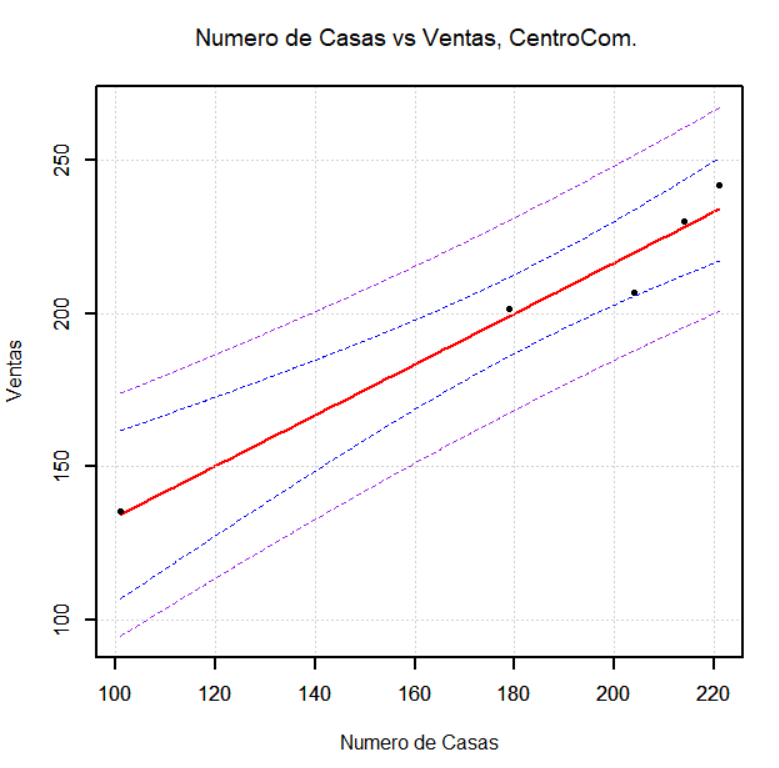
\includegraphics[scale = 0.65]{Ejercicio 4 Imagen 2 recta + int 1.png}
 \caption{Recta de regresión para las ventas en colonia utilizando como variable explicativa al número de casas. Observaciones en puntos negros, intervalo de confianza al \(95\%\) en linea punteada azul e intervalo de predicción al \(95\%\) en linea punteada púrpura.}
\label{fig:19}
\end{figure}
\begin{figure}[htb]
 \centering
 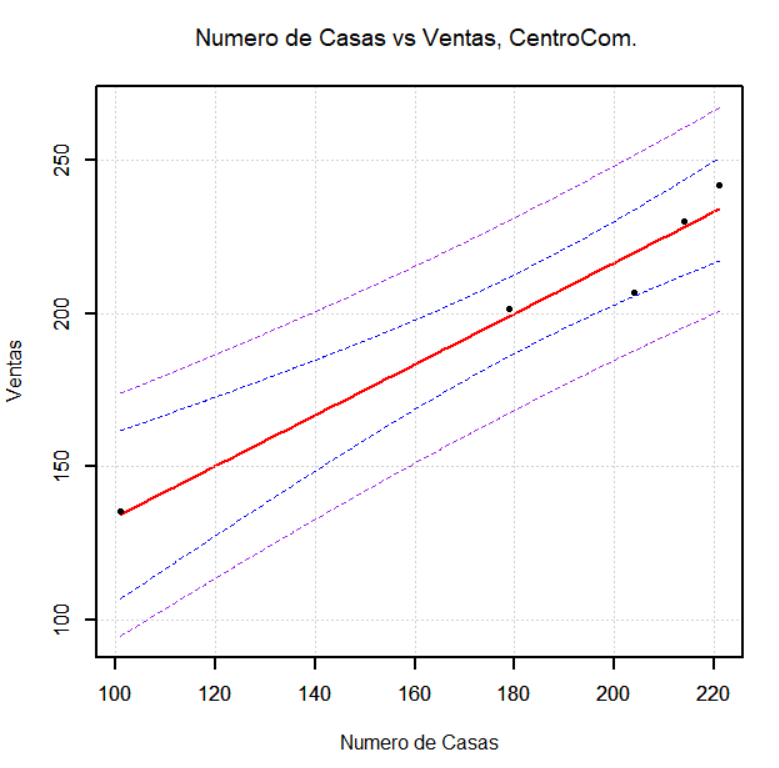
\includegraphics[scale = 0.65]{Ejercicio 4 Imagen 2 recta + int 2.png}
 \caption{Recta de regresión para las ventas en centro comercial utilizando como variable explicativa al número de casas. Observaciones en puntos negros, intervalo de confianza al \(95\%\) en linea punteada azul e intervalo de predicción al \(95\%\) en linea punteada púrpura.}
\label{fig:20}
\end{figure}
\begin{figure}[htb]
 \centering
 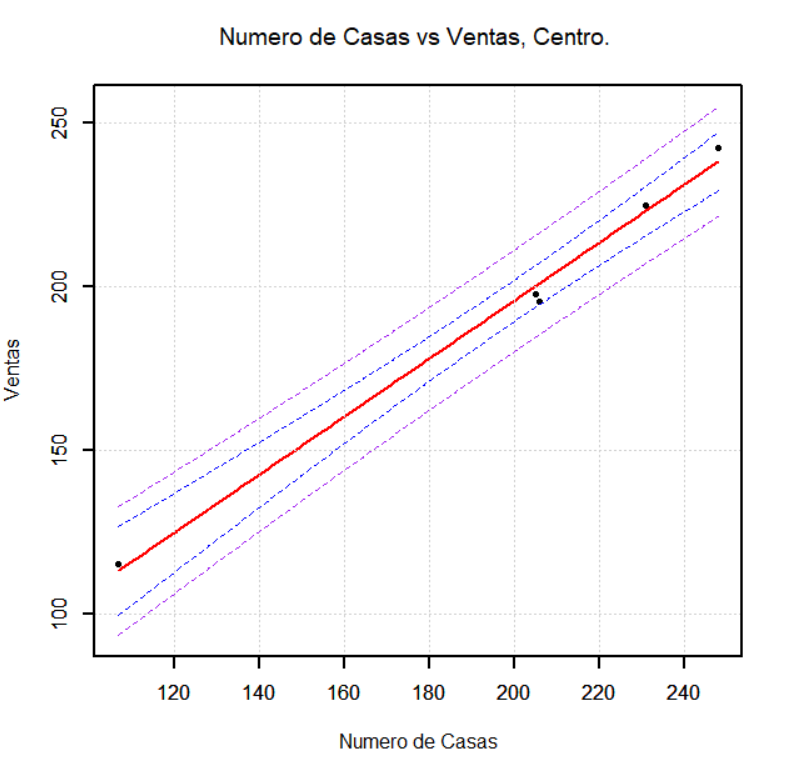
\includegraphics[scale = 0.65]{Ejercicio 4 Imagen 3 recta + int 3.png}
 \caption{Recta de regresión para las ventas en centro utilizando como variable explicativa al número de casas. Observaciones en puntos negros, intervalo de confianza al \(95\%\) en linea punteada azul e intervalo de predicción al \(95\%\) en linea punteada púrpura.}
\label{fig:21}
\end{figure}

\noindent \textbf{b)} La gráfica solicitada esta dada en la figura \ref{fig:18}, en la misma se observa que las rectas para las ventas en la colonia (recta roja) y para las ventas en el centro (recta negra), son muy parecidas, lo que nos lleva a pensar que quizás es posible combinar todos estos datos en un único modelo de regresión lineal simple. Por otro lado, las ventas en el centro comercial parecen seguir otra dinámica, ya que la recta para estas (recta azul) parece diferir bastante de las otras dos, y por ende parece apropiado considerar un modelo a parte para las mismas. Estas hipótesis serán estudiadas a profundidad en los últimos dos incisos de este ejercicio.\\

\begin{figure}[htb]
 \centering
 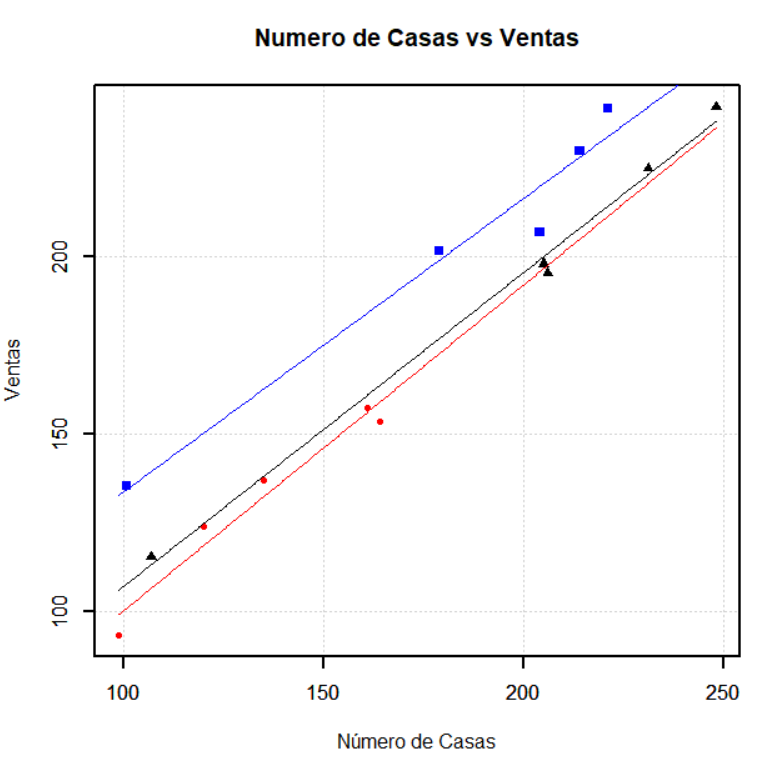
\includegraphics[scale = 0.65]{Ejercicio 4 Imagen 1 gráfico.png}
 \caption{Recta de regresión lineal para las ventas en colonia en rojo, con los datos de estas ventas en puntos rojos. Recta de regresión lineal para las ventas en centro comercial en azul, con los datos de estas ventas en cuadrados azules. Recta de regresión lineal para las ventas en centro en negro, con los datos de estas ventas en triángulos negros.}
\label{fig:18}
\end{figure}

\noindent \textbf{c)} Para \(i \in \kis{1, \hdots,15}\) sean \(D_{i1} = 1\) si la observación \(i\)-ésima tiene por localización a la colonia y \(0\) en otro caso, y sea \(D_{i2} = 1\) si la observación \(i\)-ésima tiene por localización al centro comercial y \(0\) en otro caso. Para este inciso se utilizará el siguiente modelo que contempla a las variables Dummy \(D_{1}\) y \(D_{2}\) definidas con anterioridad
\begin{equation}\label{Dummies 1}
     E[y_i | x_i, D_{i1}, D_{i2}] = \alpha_{0} + \alpha_{1}x_{i} + \alpha_{2}D_{i1} + \alpha_{3}D_{i2}, \ i = 1, \hdots, 15.\\ 
\end{equation}

El modelo anterior considera que las pendientes de las rectas para las ventas en las distintas localizaciones son iguales, pero que hay diferencias en los interceptos. Las estimaciones de los coeficientes del modelo \eqref{Dummies 1} y algunos otros detalles sobre estas estimaciones se encuentran dados en la tabla \eqref{tab:reg13} 
\begin{table}[H]
        \centering
        \begin{tabular}{@{}l@{\hskip 0.3in}r@{\hskip 0.3in}r@{\hskip 0.3in}r@{\hskip 0.3in}r@{}}
            \toprule
            Coeficiente& Estimación &\(t\)-valor& \(p\)-valor \\
            \midrule
            \(\alpha_{0}\) & 21.841 &2.552  & 0.027\\
            \(\alpha_{1}\) & 0.869 &21.452  &\(2.52\cdot10^{-10}\) \\
            \(\alpha_{2}\) & -6.864&-1.439  & 0.178\\   
            \(\alpha_{3}\) & 21.510&5.291  & \(2.56 \cdot 10^{-4}\)\\ 
            \bottomrule
        \end{tabular}
        \caption{Resultados análisis de regresión para el modelo \eqref{Dummies 1}.}
        \label{tab:reg13}
\end{table}
El \(R^2\) ajustada y el \(AIC\) de este modelo se presentan a continuación
\begin{equation}\label{AIC RRRR}
    R^2 =  0.9833, \quad AIC = 103.367.
\end{equation}

Note que bajo el modelo \eqref{Dummies 1} se tiene que 
\begin{align*}
    &\alpha_0 + \alpha_2, \ \text{es el intercepto para las ventas en la colonia.} \\
    &\alpha_0 + \alpha_3, \ \text{es el intercepto para las ventas en el centro comercial.}\\ 
    &\alpha_0, \ \text{es el intercepto para las ventas en el centro.} 
\end{align*}
De este modo se tiene que 
\begin{align*}
    &-\alpha_2 \text{ es la diferencia entre los interceptos de centro y colonia}.\\
    &-\alpha_3 \text{ es la diferencia entre los interceptos de centro y centro comercial}.\\
    &\alpha_2 - \alpha_3 \text{ es la diferencia entre los interceptos de colonia y centro comercial}.
\end{align*}
Utilizando lo anterior y las estimaciones obtenidas en la la tabla \ref{tab:reg13} se construyo la tabla \ref{tab:dif1} de la siguiente manera. Las estimaciones de las diferencias de los interceptos se obtuvieron utilizando las estimaciones de los coeficientes obtenidas en la tabla \ref{tab:reg13}. Los errores estándar se estimaron obteniendo primeramente la estimación de la matriz de covarianzas del vector de coeficientes \(\alpha=(\alpha_0,\hdots,\alpha_3)'\), la cual esta dada por la expresión \(s^2(X_1'X_1)^{-1}\) donde \(X_1 = \begin{pmatrix}1' & x_1 & D_1 & D_2\end{pmatrix}\) y \(s^2\) es la estimación de la varianza del modelo vía la suma de residuales al cuadrado, con base en ella los errores estándar se calcularon como 
\begin{equation*}
    s\sqrt{a'(X_1'X_1)^{-1}a},
\end{equation*}
con \(a\in\kis{(0,0,-1,0),(0,0,0,-1),(0,0,1,-1)}\). Por último, los valores \(t\) se calcularon como el cociente de la estimación de la diferencia entre su error estándar estimado. Por último, el \(p\)-valor se calculó como la probabilidad de que una variable aleatoria \(t(n-p)\) excediese\footnote{Esto es si \(T \sim t(n-p)\) con \(p=4\) el número de parámetros en el modelo y \(n=15\) el número de observaciones, entonces el \(p\)-valor se calculo como \(P[\abs{T} > \abs{t.valor}].\)} en valor absoluto, el valor absoluto de los valores \(t\) calculados.
\begin{table}[H]
        \centering
        \resizebox{\columnwidth}{!}{%
        \begin{tabular}{@{}l@{\hskip 0.3in}r@{\hskip 0.3in}r@{\hskip 0.3in}r@{\hskip 0.3in}r@{}}
            \toprule
            Diferencia de interceptos& Estimación & Error Estándar Estimado&\(t\)-valor& \(p\)-valor \\
            \midrule
            \(-\alpha_2\) & 6.864 & 4.770 &1.439 & 0.178 \\ 
            \(-\alpha_3\) &-21.510 & 4.065 & -5.291& \(2.557\cdot 10^{-4}\)\\ 
            \(\alpha_2-\alpha_3\) &-28.374&4.461&-6.360 & \(5.370\cdot10^{-5}\)\\ 
            \bottomrule
        \end{tabular}
        }
        \caption{Diferencias estimadas entre interceptos con errores estándar.}
        \label{tab:dif1}
\end{table}
Se destaca que de acuerdo a los \(p\)-valores en la tabla \ref{tab:dif1} la única diferencia que no resulta significativamente diferente de \(0\), bajo un nivel de significancia del \(5\%\), es la diferencia entre el intercepto del modelo para los datos de centro y colonia, lo que refuerza la hipótesis que se tenia en un inicio acerca de que pareciera razonable ajustar un solo modelo a ambos conjuntos de datos\footnote{Solo apoya, no confirma porque faltaría ver la igualdad de las estimaciones para las pendientes.}. Por otro lado, las demás diferencias si que resultan significativas lo que confirma el hecho de que un modelo distinto debe ser ajustado para los datos de ventas con localización en centro comercial. Como extra, se calculo el modelo 
\begin{equation}\label{dif222}
         E[y_i | x_i, D_{i1}, D_{i2}] = \alpha_{0}' + \alpha_{1}'x_{i} + \alpha_{2}'D_{i2}, \ i = 1, \hdots, 15.\\ 
\end{equation}
El cual considera igualdad en los interceptos para las rectas de las ventas en centro y colonia e igualdad de pendientes para todas las rectas, pero considera que el intercepto es distinto para las ventas de centro comercial. Las estimaciones para el modelo anterior se muestran en el cuadro
\begin{table}[H]
        \centering
        \begin{tabular}{@{}l@{\hskip 0.3in}r@{\hskip 0.3in}r@{\hskip 0.3in}r@{\hskip 0.3in}r@{}}
            \toprule
            Coeficiente& Estimación &\(t\)-valor& \(p\)-valor \\
            \midrule
            \(\alpha_{0}'\) &13.139 & 2.079 & 0.0597 \\
            \(\alpha_{1}'\) &0.900  & 25.302 & \(8.82\cdot 10^{-12}\)  \\
            \(\alpha_{2}'\) &24.432 & 6.648& \(2.37\cdot10^{-5}\)\\   
            \bottomrule
        \end{tabular}
        \caption{Resultados análisis de regresión para el modelo \eqref{dif222}.}
        \label{tab:reg13}
\end{table}
Por último el \(R^2\) ajustada y el \(AIC\) se presentan a continuación 
\begin{equation}\label{AIC RRRR}
    R^2 = 0.9818, \quad AIC = 103.953.
\end{equation}
Y una gráfica de las dos rectas generadas por el modelo \eqref{dif222} se muestra en la figura \eqref{fig:22}.
\begin{figure}[htb]
 \centering
 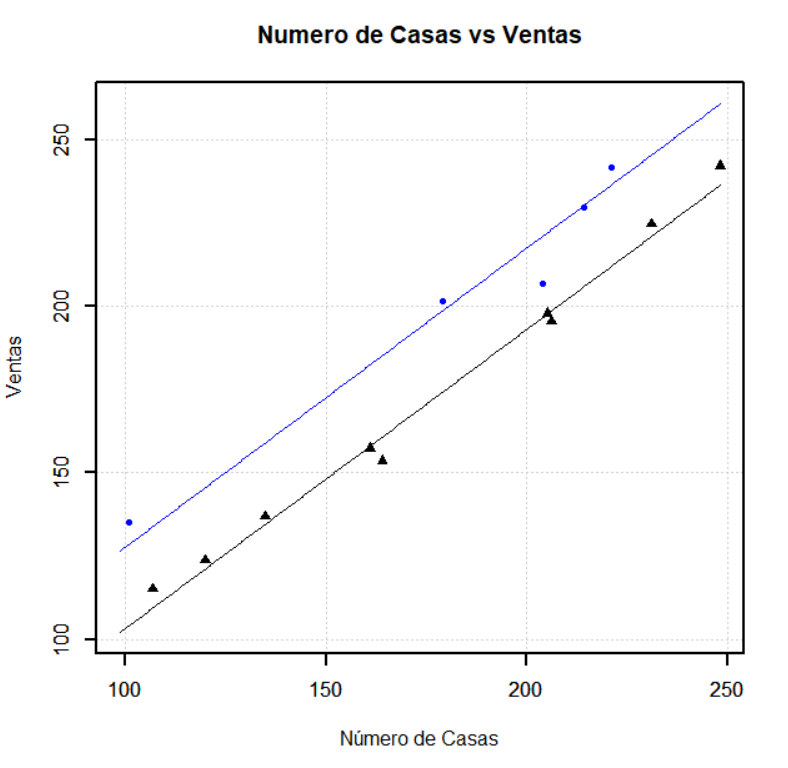
\includegraphics[scale = 0.65]{Ejercicio 4 Imagen 4 interceptos.png}
 \caption{Gráfico del modelo \eqref{dif222}}
\label{fig:22}
\end{figure}
\\

\noindent \textbf{d)} Para \(i \in \kis{1,\hdots,15}\) tome las variables \(Z_{1i} = x_i\) si \(D_{i1} = 1\) y \(Z_{1i} =0\) en otro caso, y \(Z_{i2} = x_i\) si \(D_{i2} = 1\) y \(Z_{i2} =0\) en otro caso. Para calcular la diferencia en pendientes se considerará el modelo que toma en cuenta que tanto las pendientes como los interceptos son distintos entre todas las localizaciones esto es: 
\begin{equation}\label{dididi}
E[y_i | x_i, D_{i1}, D_{i2}] = \gamma_{0} + \gamma_{1}x_{i} + \gamma_{2}D_{i1} + \gamma_{3}D_{i2}+ \gamma_{4} Z_{i1} + \gamma_{5} Z_{i2}, \ i = 1, \hdots, 15.\\
\end{equation}
El mismo nos ayudará para responder las preguntas sobre las diferencias entre las pendientes y además nos ayudará a determinar si es posible considerar un único modelo para los datos de ventas en centro y colonia. Las estimaciones para el modelo anterior se encuentran en la tabla \ref{tab:reg_234} junto con otros datos asociados a las mismas 
\begin{table}[H]
        \centering
        \begin{tabular}{@{}l@{\hskip 0.3in}r@{\hskip 0.3in}r@{\hskip 0.3in}r@{\hskip 0.3in}r@{}}
            \toprule
            Coeficiente& Estimación &\(t\)-valor& \(p\)-valor \\
            \midrule
\(\gamma_{0}\)&  18.155 &    1.423&    0.188    \\
\(\gamma_{1}\)&  0.887  &   14.275& \(1.73\cdot 10^{-7}\)\\ 
\(\gamma_{2}\)& -10.255 &   -0.482&    0.641    \\
\(\gamma_{3}\)&  32.475 &    1.774&    0.110  \\
\(\gamma_{4}\)& 0.0336  &    0.243&    0.813  \\
\(\gamma_{5}\)& -0.058  &   -0.623&    0.549  \\
            \bottomrule
        \end{tabular}
        \caption{Resultados análisis de regresión para el modelo \eqref{dididi}.}
        \label{tab:reg_234}
\end{table}
Lo primero que llama la atención acerca de este modelo, es que únicamente el coeficiente \(\gamma_{1}\) resulta significativamente distinto de \(0\), bajo un nivel de significancia del \(5\%\). Todos los demás coeficientes, en específico aquellos que marcan la diferencia en pendientes parecen ser despreciables. Al igual que en el caso anterior. Por otro lado, el \(R^2\) ajustada para este modelo y el \(AIC\) para el modelo \eqref{dididi} se presentan a continuación
\begin{equation}\label{AIC RRRR2}
    R^2 = 0.9808, \quad AIC = 106.411.
\end{equation}
Por último, una gráfica de las rectas obtenidas mediante este modelo se deja en la figura \ref{fig:23} observe que esta figura es idéntica a la presentada en el inciso b).
\begin{figure}[htb]
 \centering
 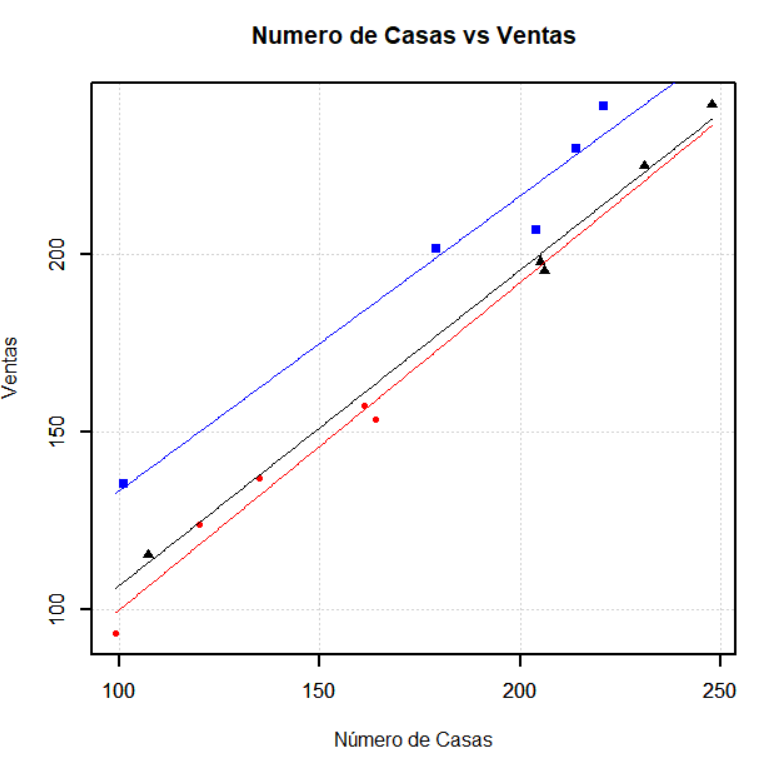
\includegraphics[scale = 0.65]{chingas a tu madre dembelé.png}
 \caption{Modelo con variables Dummy para la diferencia de pendientes.}
\label{fig:23}
\end{figure}
Note que bajo el modelo \eqref{dididi} se tiene que 
\begin{align*}
    &\gamma_1 +\gamma_4, \ \text{es la pendiente para las ventas en la colonia.} \\
    &\gamma_1 + \gamma_5, \ \text{es la pendiente para las ventas en el centro comercial.}\\ 
    &\gamma_1, \ \text{es la pendiente para las ventas en el centro.} 
\end{align*}
De este modo se tiene que 
\begin{align*}
    &-\gamma_4 \text{ es la diferencia entre las pendientes de centro y colonia}.\\
    &-\gamma_5 \text{ es la diferencia entre las pendientes de centro y centro comercial}.\\
    &\gamma_4 - \gamma_5 \text{ es la diferencia entre los pendientes de centro y centro comercial}.
\end{align*}
Utilizando lo anterior y las estimaciones obtenidas en la la tabla \ref{tab:reg_234} se construyo la tabla \ref{tab:dif2} de la siguiente manera. Las estimaciones de las diferencias de las pendientes se obtuvieron utilizando las estimaciones de los coeficientes obtenidas en la tabla \ref{tab:reg_234}. Los errores estándar se estimaron obteniendo primeramente la estimación de la matriz de covarianzas del vector de coeficientes \(\gamma=(\gamma_0,\hdots,\gamma_5)'\), la cual esta dada por la expresión \(s^2(X_2'X_2)^{-1}\) donde \(X_2 = \begin{pmatrix}1' & x & D_1 & D_2&Z_1&Z_2\end{pmatrix}\) y \(s^2\) es la estimación de la varianza del modelo vía la suma de residuales al cuadrado, con base en ella los errores estándar se calcularon como 
\begin{equation*}
    s\sqrt{a'(X_2'X_2)^{-1}a},
\end{equation*}
con \(a\in\kis{(0,0,0,0,-1,0),(0,0,0,0,0,-1),(0,0,0,0,1,-1)}\). Por otra parte, los valores \(t\) se calcularon como el cociente de la estimación de la diferencia entre su error estándar estimado. Por último, el \(p\)-valor se calculó como la probabilidad de que una variable aleatoria \(t(n-p)\) excediese\footnote{\(p=6\) el número de parámetros en el modelo y \(n=15\) el número de observaciones} en valor absoluto, el valor absoluto de los valores \(t\) calculados.
\begin{table}[H]
        \centering
        \begin{tabular}{@{}l@{\hskip 0.3in}r@{\hskip 0.3in}r@{\hskip 0.3in}r@{\hskip 0.3in}r@{}}
        \toprule
                    Diferencia de pendientes& Estimación & Error Estándar Estimado&\(t\)-valor& \(p\)-valor \\
            \midrule
            \(-\gamma_4\) &  -0.0336 &  0.138 &-0.243&    0.813 \\ 
            \(-\gamma_5\) &-0.058 & 0.093 &  0.623&    0.549\\ 
            \(\gamma_4-\gamma_5\) &0.092& 0.142&0.648& 0.533\\ 
            \bottomrule
        \end{tabular}
        \caption{Diferencias estimadas entre las pendientes con errores estándar.}
        \label{tab:dif2}
\end{table}
En el cuadro \ref{tab:dif2} se observa que ninguna diferencia en pendientes es estadísticamente significativa bajo un nivel de significancia del \(5\%\). Por último, se realizó una prueba \(F\) para contrastar la hipótesis nula \(H_0:\gamma_2 = 0\) y \(\gamma_4 = 0\) contra la hipótesis alternativa \(H_1:\gamma_2 \neq 0 \) ó \(\gamma_4 \neq 0\), esta hipótesis nula corresponde a que las rectas para centro y colonia son iguales. Tome \(K = \begin{pmatrix}0 & 0 & 1 & 0 & 0 &0\\0 & 0 & 0 & 0 & 1 &0 \end{pmatrix}'\) y observe que la hipótesis nula puede reescribirse como \(H_0: K'\gamma = 0\), además el estadístico 
\[
F = \frac{(K'\hat{\gamma})'(K'(X_2'X_2)^{-1}K)(K' \hat{\gamma})/2}{y'(I - P)y/9} \sim F_{9}^{2},
\]
bajo la hipótesis nula. Con este razonamiento se obtuvo el \(p\)-valor de \(0.636\) es decir no es posible rechazar la hipótesis de que estas dos rectas son iguales. Tomando en cuenta todo esto, se concluye que lo mejor es modelar las ventas de centro y colonia con un mismo modelo de regresión, tomar un modelo distinto para modelar las ventas en centro comercial, y considerar únicamente que existe diferencia en los interceptos entre estos dos modelos, es decir la mejor opción es considerar el modelo \eqref{dif222}.   
\end{solucion}

\newpage
\section{Referencias}
\begin{enumerate}
    \item Rawlings, J. O. (2001). Applied Regression Analysis: A Research Tool (Springer Texts in Statistics) (English Edition) (2nd ed.). Springer.
    \item Belsley, D. A., Kuh, E., Welsch, R. E. (2013). Regression Diagnostics: Identifying Influential Data and Sources of Collinearity: 546. Wiley-Interscience.
\end{enumerate}



\end{document}
